\documentclass[svgnames,t]{beamer}
\usepackage[english]{babel}
\usepackage{%
    fontspec,
    mathabx,
    pifont,
    etoolbox,
    listings,
    lstautogobble,
    tikz,
    multicol,
    moresize,
    relsize,
    array,
    booktabs,
    makecell
}

\setsansfont{Yanone Kaffeesatz}[
    UprightFont     = *-Regular ,
    BoldFont        = *-Bold ,
    BoldItalicFont  = *-Bold ,
    BoldSlantedFont = *-Bold ,
    ItalicFont      = *-Light ,
    SlantedFont     = *-Light ,
    SmallCapsFont   = *-Thin
]

%\setmonofont{Latin Modern Mono Prop}

\usetikzlibrary{
    overlay-beamer-styles,
    calc,
    positioning,
    decorations.pathreplacing,
    backgrounds, shadings,
    shapes
}

\tikzset{
    %Displaying keys
    onslide/.code args={<#1>#2}{\only<#1>{\pgfkeysalso{#2}}}, % \pgfkeysalso doesn't change the path
    scope on/.style={
        every node/.append style={visible on=#1},
        every path/.append style={visible on=#1}
    },
    %Path ending shapes
    to/.style={->,>=stealth},
    from/.style={<-,>=stealth},
    fromto/.style={<->,>=stealth},
    shorter/.style 2 args={shorten <= #1, shorten >= #2},
    %Hexagons
    hexagon/.style n args={3}{double arrow, double arrow head extend=0cm, inner sep=3pt, draw=#1, fill=#2, text=#3, thick},
    hexagon/.default={black}{gray!20}{black},
    hexagonOne/.style={hexagon={#1}{#1!30}{#1}},
    hexagonTwo/.style 2 args={hexagon={#1}{#1!#2}{#1}},
    hexagonThree/.style n args={3}{hexagon={#1}{#1!#2}{#3}},
    hexagonShade/.style n args={3}{double arrow, double arrow head extend=0cm, inner sep=3pt, thick, draw=#1, left color=#2, right color=#3},
    %General text element
    Shape/.style n args={3}{draw=#1, fill=#2, text=#3},
    genShape/.style 2 args={#1, inner sep=3pt, draw=#2, fill=#2!20, text=#2, thick},
    halo/.style={preaction={draw, #1, line width=7, -}},
}
%Colors for listings
\colorlet{background-color}{gray!20}
\colorlet{basic-color}{black}
\colorlet{keywords-color}{Goldenrod}
\colorlet{comment-color}{red!95!black}
\colorlet{strings-color}{ForestGreen}
\colorlet{builtins-color}{MediumBlue!90!black}
\colorlet{functions-color}{NavyBlue}
\colorlet{variables-color}{DarkOrange}
\colorlet{environment-color}{Gray}
\colorlet{external-color}{SteelBlue}

% https://tex.stackexchange.com/a/34000
\makeatletter
\lst@Key{countblanklines}{true}[t]%
    {\lstKV@SetIf{#1}\lst@ifcountblanklines}

\lst@AddToHook{OnEmptyLine}{%
    \lst@ifnumberblanklines\else%
       \lst@ifcountblanklines\else%
         \advance\c@lstnumber-\@ne\relax%
       \fi%
    \fi}
\makeatother

%listings set
\lstdefinestyle{MyBash}{
backgroundcolor=\color{background-color}, % choose the background color; you must add \usepackage{color} or \usepackage{xcolor}
breakatwhitespace=false,            % sets if automatic breaks should only happen at whitespace
breaklines=true,                    % sets automatic line breaking
captionpos=b,                       % sets the caption-position to bottom
deletekeywords={...},               % if you want to delete keywords from the given language
escapeinside={@|}{|@},              % if you want to add LaTeX within your code
extendedchars=true,                 % lets you use non-ASCII characters; for 8-bits encodings only,
                                    % does not work with UTF-8
frame=single,                       % adds a frame around the code
framerule=0pt,                      % Width of the frame rule
framesep=3pt,                       % separation around text
linewidth=\textwidth,               % defines the base line width for listings
xleftmargin=6mm,                    % Margin left
xrightmargin=6mm,                   % Margin right
numbers=left,                       % where to put the line-numbers; possible values are (none, left, right)
numberblanklines=false,             % suppress numbers on empty lines
countblanklines=false,              % NOT standard! Avoid counting empty lines: https://tex.stackexchange.com/a/34000
numbersep=8pt,                      % how far the line-numbers are from the code
numberstyle=\tiny\color{black},     % the style that is used for the line-numbers
rulecolor=\color{black},            % if not set, the frame-color may be changed on line-breaks within not-black text
                                    % (e.g. comments (green here))
showspaces=false,                   % show spaces everywhere adding particular underscores; it overrides 'showstringspaces'
showstringspaces=false,             % underline spaces within strings only
showtabs=false,                     % show tabs within strings adding particular underscores
stepnumber=1,                       % the step between two line-numbers. If it's 1, each line will be numbered
tabsize=2,                          % sets default tabsize to 2 spaces
title=\lstname,                     % show the filename of files included with \lstinputlisting; also try caption instead of title
%
%Base style for this presentation 
keepspaces=true,                    % keeps spaces in text, useful for keeping indentation of code
                                    % (possibly needs columns=flexible)
language=bash,
basicstyle=\ttfamily\scriptsize\color{basic-color},
keywordstyle=\color{keywords-color},
stringstyle=\color{strings-color},
commentstyle=\color{comment-color},
morestring=[b][\color{strings-color}]{"},
morestring=[d][\color{strings-color}]{'},
moredelim=[is][\color{basic-color}]{|+}{+|}, % I will use this for terminal output
literate={`}{\textasciigrave}1, % https://tex.stackexchange.com/a/466224/128737
literate={~}{{\textasciitilde}}1,
% literate=% literate={<replace>}{<replacement text>}{<width>}
%   {\#define}{{{\color{CarnationPink}\#define}}}{6}
%   {\#include}{{{\color{CarnationPink}\#include}}}{7},
alsoletter=0123456789![]/\{\}.:+, % This to mark the symbols in keyword/emph[5] to be highlighted (otherkeywords does not work i.e. it highlights also in comments!) -> manual at page 45
morekeywords={if, then, else, elif, fi, case, esac, for, select, while, until, do, done, in, function, time, [[, ]], \{, \}, !, coproc}, %https://askubuntu.com/a/513712
emph=[1]{CreateListOfFiles, LevelOne, LevelTwo, LevelThree, Test, SecondsToTimeStringWithDays, ExampleFunction,
         ExampleFunction_implementation, ExtractColumnFromFile, CalculateSizeOfFiles, ReportOnLargestDirectories,
         CountTill5From, FifthElementOf, CreateAuxiliaryFiles, CleanAuxiliaryFiles, Failure, FailureMsg, Simulation},
emphstyle=[1]{\color{functions-color}}, %Functions
emph=[2]{variableName, invisibleVariable, prefix, day, today, song, aVar, bVar, langRegex, deadline, now,
         index, file, fgbg, color, reference, files, array, message, entry, index, dict, key, flag, line, inputTime,
         days, hours, minutes, seconds, globalVar, pid, extglobSet, counter, filename, extension},
emphstyle=[2]{\color{variables-color}}, %Variables
emph=[4]{PATH, SHELL, IFS, BASH_ALIASES, BASH_REMATCH, PS3, REPLY, HOME, LANGUAGE, EDITOR, PIPESTATUS, PWD, FUNCNEST,
         DIRSTACK, PWD, OLDPWD, SHELLOPTS, BASHOPTS, TIMEFORMAT, COMP_CWORD, COMP_LINE, COMP_POINT, COMP_TYPE, COMP_KEY,
         COMP_WORDBREAKS, COMP_WORDS, COMPREPLY, INPUTRC},
emphstyle=[4]{\color{environment-color}}, %Environment variables
emph=[5]{alias, bg, bind, break, builtin, cd, command, compgen, complete, continue, declare, dirs, disown, echo, enable, eval,
         exec, exit, export, false, fc, fg, getopts, hash, help, history, jobs, kill, let, local, logout, popd, printf, pushd, pwd,
         read, readonly, return, set, shift, shopt, source, suspend, test, times, trap, true, type, typeset, ulimit, umask,
         % case, if, until, while  % <--- these built-in are keywords and I leave them highlighted as such
         unalias, unset, wait, :, ., [, ]},
emphstyle=[5]{\color{builtins-color}}, %Shell built-in
emph=[6]{man, apropos, ls, rm, g++, chmod, cp, awk, sed, cut, perl, args, date, grep, sleep, tput, seq, cat, wc, sort, tail,
         head, sdiff, tar, mktemp, mkdir, ps, emacs, systemd, timeout, parallel, xargs, gnuplot, pdflatex, vi, ping, bash,
         egrep, shuf, stat, find, fgrep, bc, tr, paste, expr, diff, touch},
emphstyle=[6]{\color{external-color}}, %(External) commands
emph=[7]{},
emphstyle=[7]{\color{variables-color}}, %Class for local variables (usually with bad names)
emph=[8]{},
emphstyle=[8]{\color{builtins-color}}, %Class for local commands (usually with bad names)
%
%Additional customizations
belowskip=-7mm,
aboveskip=3pt,
autogobble=true, % lstautogobble needed!
}

\lstnewenvironment{Bash}[1][] %I will rarely use this because putting a $ in it as prompt breaks down TeXclipse highlight syntax!
    {\lstset{style=MyBash, #1}}
    {}

\def\bash{\lstinline[style=MyBash, basicstyle=\ttfamily\color{black}]}

%This additional style is to just print odd numbers (NOTE: style keyword can be repeated and it is cumulative!)
\lstdefinestyle{oddnumbers}{
    stepnumber=2,
    firstnumber=0,
    numberstyle={\tiny\color{black}\ifodd\value{lstnumber}\relax\else\refstepcounter{lstnumber}\fi\tiny\color{black}\ifodd\value{lstnumber}\relax\else\refstepcounter{lstnumber}\fi}
}

%This additional style is to just print odd numbers (NOTE: style keyword can be repeated and it is cumulative!)
\lstdefinestyle{smaller}{
    basicstyle={\linespread{1.2}\ttfamily\ssmall\color{basic-color}}
}

\newcommand<>{\tc}[2]{\textcolor#3{#1}{#2}}
\newcommand{\tikzmark}[1]{\tikz[overlay,remember picture, baseline=-0.5ex] \node at (0,0) (#1) {};}
\newcommand{\URLsymbol}[2][white]{%
    \begin{tikzpicture}[every path/.style={line width=3, rounded corners, #2}]
        \pgfmathsetmacro{\longSide}{0.9}
        \pgfmathsetmacro{\shortSide}{0.3}
        \draw[rotate=45, xshift=0.5*\longSide cm]       (0,0) rectangle (\longSide, \shortSide);
        \draw[rotate=45, halo=#1, #2!50]                   (0,0) rectangle (\longSide, \shortSide);
        \draw[rotate=45, halo=#1, xshift=0.5*\longSide cm] (0, 0.5*\shortSide) -- (0,0) -- (\longSide, 0) -- (\longSide, 0.5*\shortSide);
    \end{tikzpicture}
}
\NewDocumentCommand{\URL}{ O{black} m m O{BGLIGHT} }%
{%
    \raisebox{-0.4ex}{\resizebox{!}{2ex}{\URLsymbol[#4]{#1}}}{\href{#2}{\textcolor{#1}{#3}}}
}

\NewDocumentCommand{\addSection}{ m O{} m m }%
{%
    \setbeamertemplate{section page}[Iceland][#2]{#3}{#4}
    \section{#1}
}

\makeatletter
\newcommand*\keystroke[1]
{%
    \begin{tikzpicture}[baseline=($(key.base)!0.8!(key.south)$), very thin]%
        \pgfmathsetlengthmacro{\textHeight}{0.9*\f@size}
        \pgfmathsetlengthmacro{\textHeightPlus}{1.25*\textHeight}
        \pgfmathsetlengthmacro{\roundedSmall}{0.2}
        \pgfmathsetlengthmacro{\roundedLarge}{0.4}
        \pgfmathsetlengthmacro{\dl}{0.5\pgflinewidth}
        \node[font=\sffamily, inner xsep=2pt, inner ysep=1pt] (text) {\scalebox{1.2}[0.75]{\textsmaller[2]{#1\strut}}};
        \node[rounded corners=\roundedLarge, minimum size=\textHeight, anchor=north west] (key) at (text.north west){};
        \node[rounded corners=\roundedSmall, minimum size=\textHeightPlus] (frame) at ($(key.center)!0.05!(key.south)$){};
        \path coordinate (keyNW) at ($(key.north west)+(\roundedLarge,-\dl)$)
              coordinate (keyNE) at ($(key.north east)-(\roundedLarge,+\dl)$)
              coordinate (keyEN) at ($(key.north east)-(-\dl,\roundedLarge)$)
              coordinate (keyES) at ($(key.south east)+(+\dl,\roundedLarge)$)
              coordinate (keySE) at ($(key.south east)-(\roundedLarge,+\dl)$)
              coordinate (keySW) at ($(key.south west)+(\roundedLarge,-\dl)$)
              coordinate (keyWS) at ($(key.south west)+(+\dl,\roundedLarge)$)
              coordinate (keyWN) at ($(key.north west)-(-\dl,\roundedLarge)$)
              coordinate (frameNW) at ($(frame.north west)+(\roundedSmall,-\dl)$)
              coordinate (frameNE) at ($(frame.north east)-(\roundedSmall,+\dl)$)
              coordinate (frameEN) at ($(frame.north east)-(+\dl,\roundedSmall)$)
              coordinate (frameES) at ($(frame.south east)+(-\dl,\roundedSmall)$)
              coordinate (frameSE) at ($(frame.south east)-(\roundedSmall,-\dl)$)
              coordinate (frameSW) at ($(frame.south west)+(\roundedSmall,+\dl)$)
              coordinate (frameWS) at ($(frame.south west)+(+\dl,\roundedSmall)$)
              coordinate (frameWN) at ($(frame.north west)-(-\dl,\roundedSmall)$);
        \foreach \n in {NW,NE,EN,ES,SE,SW,WS,WN}{
            \draw[line cap=round, ultra thin] (key\n) -- (frame\n);
        }
        \begin{scope}[on background layer]
            \node[draw, rounded corners=\roundedSmall, minimum size=\textHeightPlus, fill=fg] at ($(key.center)!0.05!(key.south)$){};
            \node[draw, rounded corners=\roundedLarge, lower right=gray!20, lower left=gray!50, upper right=gray!50, upper left=gray!80, minimum size=\textHeight, anchor=north west] at (text.north west){};
            \fill [gray!70!bg] (keyNW) -- (keyNE) -- (frameNE) -- (frameNW) -- cycle;
            \fill [gray!50!bg] (keyWS) -- (keyWN) -- (frameWN) -- (frameWS) -- cycle;
            \fill [gray!30!bg] (keyES) -- (keyEN) -- (frameEN) -- (frameES) -- cycle;
            \fill [gray!10!bg]  (keySW) -- (keySE) -- (frameSE) -- (frameSW) -- cycle;
        \end{scope}
  \end{tikzpicture}%
}
\makeatother

\newcommand{\Remark}[2][1mm]
{%
    \hspace{#1}{\tiny\{~#2~\}}%
}

\newcommand{\FrameRemark}[2][1-]%
{%
    \begin{tikzpicture}[remember picture, overlay]
        \node[font=\tiny, anchor=south, visible on=<#1>] at (current page.south) {#2};
    \end{tikzpicture}
}

\newcommand{\MakeEnumerateBox}[1]%
{%
    \hbox{%
      \usebeamerfont*{item projected}%
      \usebeamercolor[bg]{item projected}%
      \vrule width2.25ex height1.85ex depth.4ex%
      \hskip-2.25ex%
      \hbox to2.25ex{%
        \hfil%
        \color{fg}#1%
        \hfil}%
    }%
}

\renewcommand{\checkmark}[1][PS]{\tc{#1}{\ding{51}}}
\newcommand{\crossmark}[1][PT]{\tc{#1}{\ding{55}}}

\def\quizOverlay{1}
\newcounter{QuizNumber}
\resetcounteronoverlays{QuizNumber}% To avoid the counter being increased by overlays
\newenvironment{quiz}[2][1]{%
    \edef\tmpNumber{\numexpr #1 +1\relax}%
    \gdef\quizOverlay{\the\tmpNumber}%
    \stepcounter{QuizNumber}%
    \medskip%
    % mbox to avoid newline after hbox of enumerate
    \mbox{\MakeEnumerateBox{\theQuizNumber}}\enspace #2%
    \begin{itemize}%
}{%
    \end{itemize}%
    \bigskip%
}

\newcommand{\wrongChoice}[1]%
{%
    \item[\alt<\quizOverlay->{\crossmark}{$\bullet$}] #1
}

\newcommand{\correctChoice}[1]%
{%
    \item[\alt<\quizOverlay->{\checkmark}{$\bullet$}] #1
}

\graphicspath{{Figures/}{Figures/Iceland}}
\makeatletter
\newif\ifgraphicexist

\catcode`\*=11
\newcommand\IfImageCanBeIncluded[1]{% Taken from https://tex.stackexchange.com/a/567990/128737
    \begingroup
        \global\graphicexisttrue
        \ifx\detokenize\@undefined\else
            \edef\Gin@extensions{\detokenize\expandafter{\Gin@extensions}}%
        \fi
        \let\input@path\Ginput@path
        \expandafter\filename@parse\expandafter{#1}%
        \ifx\filename@ext\Gin@gzext
            \expandafter\filename@parse\expandafter{\filename@base}%
            \ifx\filename@ext\relax
                \let\filename@ext\Gin@gzext
            \else
                \edef\Gin@ext{\Gin@ext\Gin@sepdefault\Gin@gzext}%
            \fi
        \fi
        \ifx\filename@ext\relax
            \@for\Gin@temp:=\Gin@extensions\do{%
                \ifx\Gin@ext\relax
                    \Gin@getbase\Gin@temp
                \fi}%
        \else
            \Gin@getbase{\Gin@sepdefault\filename@ext}%
            \ifx\Gin@ext\relax
                \global\graphicexistfalse
                \let\Gin@savedbase\filename@base
                \let\Gin@savedext\filename@ext
                \edef\filename@base{\filename@base\Gin@sepdefault\filename@ext}%
                \let\filename@ext\relax
                \@for\Gin@temp:=\Gin@extensions\do{%
                    \ifx\Gin@ext\relax
                        \Gin@getbase\Gin@temp
                    \fi}%
                    \ifx\Gin@ext\relax
                        \let\filename@base\Gin@savedbase
                        \let\filename@ext\Gin@savedext
                    \fi
                \fi
                \ifx\Gin@ext\relax
                    \global\graphicexistfalse
                    \def\Gin@base{\filename@area\filename@base}%
                    \edef\Gin@ext{\Gin@sepdefault\filename@ext}%
                \fi
        \fi
        \ifx\Gin@ext\relax
            \global\graphicexistfalse
        \else
        \@ifundefined{Gin@rule@\Gin@ext}%
            {\global\graphicexistfalse}%
            {}%
        \fi
        \ifx\Gin@ext\relax 
            \gdef\imageextension{unknown}%
        \else
            \xdef\imageextension{\Gin@ext}%
        \fi 
    \endgroup 
    \ifgraphicexist
        \expandafter \@firstoftwo
    \else
        \expandafter \@secondoftwo
    \fi
}
\catcode`\*=12
\makeatother

% Compile with or without photos
\newif\ifCompileWithPhotos
\CompileWithPhotostrue

% Compile with or without photos
\newif\ifAddLinkToTOC
\AddLinkToTOCtrue

\mode<presentation>
{
    \usetheme{Relax}
    \defbeamertemplate{footline}{Empty}{}
    \setbeamersize{text margin left=8mm,text margin right=8mm}
    %\setbeamerfont{section title}{size=\Huge}
    \defbeamertemplate*{section page}{Iceland}[3][]
    {
        \begin{tikzpicture}[overlay,remember picture, every node/.style={inner sep=0pt}]
            \usebeamercolor{section page background canvas}
            \fill[bg] (current page.south west) rectangle (current page.north east);
            \node[text depth=0.5ex, anchor=west] () (sectionTitle) at ($(current page.north west)+(5mm,-8mm)$)
                  {\usebeamerfont{section title}\usebeamercolor[fg]{section title}\insertsectionhead};
            \node[anchor=north east, inner sep=0] (plan) at ($(current page.north east)-(1mm,1mm)$) {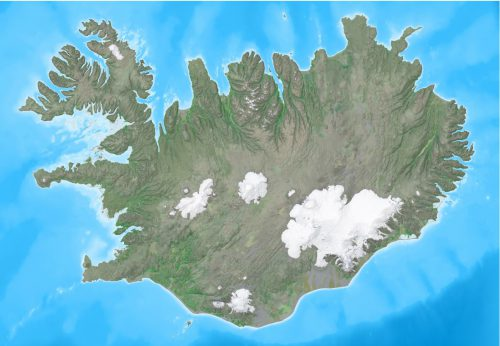
\includegraphics[width=0.21\textwidth, clip, trim=0 0 0 1mm]{Map}};
            \node[anchor=north] (photo) at ($(plan.south west)!0.5!(sectionTitle.south west |- plan.south)-(0,1mm)$) {
                \ifCompileWithPhotos%
                    \IfImageCanBeIncluded{#2}{%
                        \includegraphics[width=0.85\textwidth]{#2}
                    }{%
                        \includegraphics[width=0.75\textwidth]{example-image-a}
                    }
                \else
                    \includegraphics[width=0.75\textwidth]{example-image-a}
                \fi
            };
            \node[text depth=0.5ex, below = 2mm of photo.south east, anchor=north east, xshift=-2pt]{#3};
            \ifthenelse{\isempty{#1}}{}%
            {
                \begin{scope}[x={($ (plan.south east) - (plan.south west) $ )},y={( $ (plan.north west) - (plan.south west)$ )}, shift={(plan.south west)}]
                    %\draw[help lines,xstep=.1,ystep=.1] (0,0) grid (1,1);
                    \node[anchor=south, inner sep=0] at (#1) {
\includegraphics[width=2mm]{Pin}};
                \end{scope}
            }
            \ifCompileWithPhotos
                \IfImageCanBeIncluded{#2}{%
                    \node[rotate=90, anchor=west, font=\ssmall] at ($(current page.south east)+(-2mm,1mm)$) {{\raisebox{-2mm}{\Large\textcopyright}} Photo: All rights are reserved};
                }{}
            \fi
        \end{tikzpicture}
    }
    %Add a link to table of content on frames with a footline
    \addtobeamertemplate{footline}{}{%
        \ifAddLinkToTOC%
            \begin{tikzpicture}[remember picture,overlay]
                %xelatex needs \XeTeXLinkBox, won't create a link unless it
                %finds text --- rules don't work without \XeTeXLinkBox.
                %Still builds correctly with pdflatex and lualatex
                \node[anchor=south east, inner sep=2pt] at (current page.south east) {\hyperlink{toc}{\XeTeXLinkBox{
\includegraphics[width=3mm]{TOC}}}};
            \end{tikzpicture}%
        \fi%
    }%
}

\makeatletter
\AtBeginSection[]% <- Empty optional argument, do nothing for \section*
{%
    \ifnum\beamer@tocsectionnumber>0%
        \begin{frame}[plain, noframenumbering]{}
             \sectionpage
        \end{frame}
    \fi
}
\makeatother

%Append code to put third CSC logo on titlepage
\appto\titlepage{%
    \begin{tikzpicture}[remember picture, overlay]
        \node[anchor=south] at (current page.south) {
\includegraphics[width=25mm]{LogoCSC}};
    \end{tikzpicture}
}

%===============================================================%
\title{Introduction to Bash scripting language}
\author{Alessandro Sciarra \texorpdfstring{\\}{} {\tiny Z02~--~Software Development Center}}
\institute{Organised by the CSC Frankfurt}
\titlegraphic{
\includegraphics[width=20mm]{LogoCRC}}
\titlepagelogo{
\includegraphics[width=20mm]{LogoGoethe}}
%===============================================================%


%===================%
\subtitle{Day 3}
\date{09.10.2019}
%===================%

\begin{document}
    %-------------------------------%
%  Author: Alessandro Sciarra   %
%    Date: 21 Aug 2019          %
%-------------------------------%

%~~~~~~~~~~~~~~~~~~~~~~~~~~~~~~~~~~~~~~~~~~~~%
\begin{frame}[plain,noframenumbering]
    \titlepage
\end{frame}
%~~~~~~~~~~~~~~~~~~~~~~~~~~~~~~~~~~~~~~~~~~~~%
\begin{frame}[plain,noframenumbering]{Topics of the day}
    \medskip
    \begin{columns}[t]
        \begin{column}{.45\textwidth}
            \hspace*{4mm}
            \begin{minipage}[t][0.45\textheight]{\textwidth}
                \tableofcontents[sections={1-3}]
            \end{minipage}
        \end{column}
        \begin{column}{.45\textwidth}
            \begin{minipage}[t][0.45\textheight]{\textwidth}
                \tableofcontents[sections={4-}]
            \end{minipage}
        \end{column}
    \end{columns}
    \vspace{6mm}
    \begin{varblock}{example}[0.9\textwidth]{You already know almost everything}
        Today we will complete the picture about bash for almost all purposes, discovering some useful features for your daily work!
    \end{varblock}
\end{frame}
%~~~~~~~~~~~~~~~~~~~~~~~~~~~~~~~~~~~~~~~~~~~~%

    \addSection{Compound commands}{example-image-a}{distribution image}
    %-------------------------------%
%  Author: Alessandro Sciarra   %
%    Date: 21 Aug 2019          %
%-------------------------------%

%~~~~~~~~~~~~~~~~~~~~~~~~~~~~~~~~~~~~~~~~~~~~%
\begin{frame}{Compound commands}
    \begin{itemize}
        \item \only<2>{\pgfsetfillopacity{0.5}}\bash{if} statements\tikzmark{doneStart}
        \item \bash{for} loops
        \item \bash{while}, \bash{until} loops
        \item \bash{[[} keyword
        \item \bash{case}, \bash{select} constructs\tikzmark{doneEnd}\pgfsetfillopacity{1}\medskip
        \item \tc<2>{PP}{Subshells}\tikzmark{nowStart}
        \item \tc<2>{PP}{Command grouping}
        \item \tc<2>{PP}{Arithmetic evaluation}\tikzmark{nowEnd}\\[-0.5ex] {\tiny\{~Slightly different from the \PQ{Arithmetic expansion} we already discussed~\}}\medskip
        \item \tc<2>{PB}{[Functions]\tikzmark{fcts}} {\tiny\{~Discussed in detail in a separate section~\}}
    \end{itemize}
    \begin{tikzpicture}[remember picture, overlay]
        \begin{scope}[scope on=<2>]
            \draw[very thick, decorate, decoration={brace,amplitude=6pt}] (doneStart -| doneEnd) ++(8mm,1mm) -- ($(doneEnd)+(8mm,-1mm)$) 
                      node[midway, right=3mm, text width=40mm, align=center] {Already discussed in details};
            \draw[very thick, decorate, decoration={brace,amplitude=6pt}, PP] (nowStart -| nowEnd) ++(8mm,1mm) -- ($(nowEnd)+(8mm,-1mm)$) 
                      node[midway, right=3mm, text width=40mm, align=center, text=PP] {What we are going to discuss};
            \path[from, PB] ($(fcts)-(6.8mm,3mm)$) edge[out=270, in=180] node[pos=1, right, font=\footnotesize, text=PB] {Strictly speaking not a compound command, but they work in a similar way} ++(2cm,-1cm);
        \end{scope}
    \end{tikzpicture}
\end{frame}
%~~~~~~~~~~~~~~~~~~~~~~~~~~~~~~~~~~~~~~~~~~~~%
\begin{frame}{Subshells}
    \vspace{-8mm}
    \begin{overlayarea}{\textwidth}{0.7\textheight}
        \begin{varblock}{}[0.8\textwidth]{Definition}
            A subshell is \textbf{a child process} but it is one \textbf{that inherits more than a normal external command} does.
            It can see all the variables of your script, not just the ones that have been exported to the environment.
        \end{varblock}
        \begin{varblock}{quote}[0.88\textwidth]{Unix Process}<only@1>
            Every process on a Unix system has its own parcel of memory, for holding its variables, its file descriptors, its copy of the Environment inherited from its parent process, and so on.
            The changes to the variables (and other private information) in one process do not affect any other processes currently running on the system.
        \end{varblock}
        \begin{varblock}{alerted}[0.6\textwidth]{Use them consciously}<only@1>
            Forking a subshell leads to a speed penalty which often is irrelevant but which you should keep in mind!
        \end{varblock}
        \begin{itemize}[<2>]
            \item It is explicitly forced using the parenthesis \PB{\texttt{(\ldots)}}
            \item Changes e.g. to variables done in a subshell are not remembered when exiting the subshell: A subshell can be thought as a temporary shell!
            \item There are many instances in which a shell creates a subshell without parentheses being placed by the programmer
                  \begin{itemize}
                      \item \PP{In pipelines} $\;\longleftarrow\;$ \alert{\textbf{Every command in a pipeline is run in its own subshell!}}
                      \item \PP{In command substitution}
                      \item Executing other programs or scripts
                      \item In any external command that executes new shells (e.g. \bash{awk}, \bash{sed}, \bash{perl})
                      \item In process substitution
                      \item In backgrounded commands and coprocs
                  \end{itemize}
        \end{itemize}
    \end{overlayarea}
    \FrameRemark[2]{From Bash v4.2 the shell option \texttt{lastpipe} can be enabled so that the last command in a pipeline is not run in a subshell.}
\end{frame}
%~~~~~~~~~~~~~~~~~~~~~~~~~~~~~~~~~~~~~~~~~~~~%
\begin{frame}[fragile]{Subshells: Examples}
    \begin{lstlisting}[style=MyBash]
        # Changes in a subshell do not propagate back
        $ aVar="Hello"; pwd
        /home/sciarra/Documents
        $ ( aVar="Goodbye"; echo "${aVar}" ); echo "${aVar}"
        |+Goodbye+|
        |+Hello+|
        $ ( cd /tmp; pwd ); pwd
        |+/tmp
        /home/sciarra/Documents+|
        # It is often a feature to take advantage of!
        $ (cd /tmp || exit 1; tar ...)
        $ (source ~/AuxiliaryBashTools.bash; ...)
        # In a subshell the script variable are accessible
        $ ( echo "${aVar} from the subshell" )
        |+Hello from the subshell+|
        # Implicit subshells: be aware of them!
        $ echo "Goodbye" | read aVar; echo "${aVar}"
        |+Hello+|
        $ read aVar <<< "Goodbye"; echo "${aVar}"; unset aVar
        |+Goodbye+|
    \end{lstlisting}
    \FrameRemark{\URL[PB]{http://mywiki.wooledge.org/BashFAQ/024}{Advanced reading} about pipelines and subshells: Why can't I pipe data to read?}
\end{frame}
%~~~~~~~~~~~~~~~~~~~~~~~~~~~~~~~~~~~~~~~~~~~~%
\begin{frame}[fragile]{Command grouping}{We already said something about it, let us go through once again}
    \vspace{-4mm}
    \begin{overlayarea}{\textwidth}{0.7\textheight}
        \begin{itemize}
            \item Commands may be grouped together using curly braces \PB{\texttt{\{\ldots\}}}
            \item Command groups allow a collection of commands to be considered as a whole with regards to redirection and control flow
            \item All compound commands such as \bash|if| statements and \bash|while| loops do this as well, but command groups do \textbf{only} this
            \item Command groups are executed in the same shell as everything else, NOT in a new one!
        \end{itemize}
        \begin{lstlisting}[style=MyBash, numbers=none]
            $ { echo "$(date)"
            >   rsync -av |+.+| /backup; echo "$(date)";@|\tikzmark{sc}|@ } >backup.log 2>&1
        \end{lstlisting}
        \smallskip
        \begin{varblock}{quote}[0.9\textwidth]{}<only@1>
            The above example truncates and opens the file backup.log on stdout, then points stderr at where stdout is currently pointing (backup.log), then runs each command with those redirections applied.
            The file descriptors remain open until all commands within the command group complete before they are automatically closed.
            This means backup.log is only opened a single time, not opened and closed for each command.
        \end{varblock}
        \begin{tikzpicture}[remember picture, overlay]
            \begin{scope}[scope on=<2->]
                \path[from, PT] ($(sc)-(0.9mm,1.5mm)$) edge[out=270, in=90] node[pos=1, below, font=\large, text=PT] (q) {Why is this semicolon absolutely \textbf{mandatory}?} ++(0cm,-1cm);
            \end{scope}
            \node[visible on=<3->, text width=5.6cm, align=center, below = 1mm of q, font=\scriptsize] {Because otherwise the closing curly bracket would be a argument of the final \mbox{command} in the group, \bash|echo| in this case};
        \end{tikzpicture}
    \end{overlayarea}
\end{frame}
%~~~~~~~~~~~~~~~~~~~~~~~~~~~~~~~~~~~~~~~~~~~~%
\begin{frame}[fragile]{Arithmetic evaluation: The \bash|let| builtin}
    \vspace{-4mm}
    \begin{itemize}
        \item Sometimes we want to do arithmetic instead of string operations
        \item One way to do so is to use the \bash|let| builtin
              \begin{lstlisting}[style=MyBash, style=oddnumbers, aboveskip=2mm, belowskip=-6mm]
                  $ aVar=4+5; echo "${aVar}"
                  |+4+5+|
                  $ let aVar=4+5; echo "${aVar}"; unset aVar
                  |+9+|
              \end{lstlisting}
        \item However, it requires quotes to use arithmetic operators $\quad${\tiny\{~\bash|help let|~\}}
              \begin{lstlisting}[style=MyBash, style=oddnumbers, aboveskip=2mm, belowskip=-6mm]
                  $ let aVar=2<3
                  |+bash: 3: No such file or directory+|
                  $ let aVar='2<3'; echo "${aVar}"; unset aVar
                  |+1+|
              \end{lstlisting}
        \item \bash|let| accepts more than one expression
              \begin{lstlisting}[style=MyBash, style=oddnumbers, aboveskip=2mm, belowskip=-6mm]
                  $ let aVar='2<3' bVar=3*7; echo "${aVar} ${bVar}"
                  |+1 21+|
                  $ unset aVar bVar
              \end{lstlisting}
        \item If the last expression evaluates to 0, \bash|let| returns 1; \bash|let| returns 0 otherwise.
    \end{itemize}
\end{frame}
%~~~~~~~~~~~~~~~~~~~~~~~~~~~~~~~~~~~~~~~~~~~~%
\begin{frame}[fragile]{Arithmetic evaluation: The command grouping \PB{\texttt{((\ldots))}}}
    \vspace{-4mm}
    \begin{overlayarea}{\textwidth}{0.7\textheight}
        \begin{itemize}
            \item<only@1> \PB{\texttt{(( expression ))}} $\;$is  equivalent to$\;$ \bash|let "expression"|
            \item<only@1> No quote is needed in it, since only arithmetic operations are there performed
            \item<only@1> However, only one expression can be evaluated (not bad for the exit code)
                  \begin{lstlisting}[style=MyBash, style=oddnumbers, aboveskip=2mm, belowskip=-6mm]
                      $ (( aVar=7*3**2 )); echo "${aVar}"
                      |+63+|
                      $ (( aVar=1+${aVar}/20 )); echo "${aVar}"; unset aVar
                      |+4+|        # '${}' not really needed@|$^\star$|@
                  \end{lstlisting}
            \item<only@1> Although not a compound command, the arithmetic substitution uses the same syntax
                  \begin{lstlisting}[style=MyBash, style=oddnumbers, aboveskip=2mm, belowskip=-6mm]
                      $ (( aVar=7*3**2 )); echo "${aVar}"
                      |+63+|
                      $ echo "aVar=$(( 7*3**2 ))"; unset aVar
                      |+63+|
                  \end{lstlisting}
            \item<only@1> Assignments in arithmetic substitution work but are confusing and should be avoided!
                  \begin{lstlisting}[style=MyBash, style=oddnumbers, aboveskip=2mm, belowskip=-6mm]
                      $ echo "_${bVar}_ $(( bVar=7*3**2 )) _${bVar}_"
                      |+__ 63 _63_+|
                  \end{lstlisting}
            \item<only@2> Arithmetic evaluation is very helpful in combination with conditionals
                  \begin{lstlisting}[style=MyBash, aboveskip=2mm, belowskip=-6mm]
                      $ ((aVar=(5+2)*3))
                      $ if ((aVar == 21)); then
                      >   echo 'Blackjack!'
                      > fi
                      |+Blackjack!+|
                  \end{lstlisting}
            \item<only@2> Because the inside of \PB{\texttt{((\ldots))}} is C-like, a variable (or expression) that \PP{evaluates to zero} will be considered \PP{false} for the purposes of the arithmetic evaluation.
                  Then, because the evaluation is false, it will \PP{exit with a status of 1}.
                  Likewise, if the expression inside \PB{\texttt{((\ldots))}} \PS{is non-zero}, it will be considered \PS{true}; and since the evaluation is true, it will \PS{exit with status 0}.
                  \begin{lstlisting}[style=MyBash, aboveskip=2mm, belowskip=-6mm]
                      $ flag=0  # no error
                      $ while read line; do
                      >   if [[ ${line}= *err* ]]; then flag=1; fi
                      > done < inputfile
                      $ if ((flag)); then echo 'Houston, we have a problem!'; fi
                  \end{lstlisting}
        \end{itemize}
    \end{overlayarea}
    \FrameRemark[1]{$^\star$Using the \texttt{\$\{\}} makes Bash use \bash|''| for uninitialised variables and might trigger errors (\texttt{0} is used for uninitialised variables referenced without \texttt{\$\{\}} syntax).}
\end{frame}
%~~~~~~~~~~~~~~~~~~~~~~~~~~~~~~~~~~~~~~~~~~~~%


    \addSection{Functions}{example-image-a}{distribution image}
    %-------------------------------%
%  Author: Alessandro Sciarra   %
%    Date: 25 Sep 2020          %
%-------------------------------%

%~~~~~~~~~~~~~~~~~~~~~~~~~~~~~~~~~~~~~~~~~~~~%
\begin{frame}{Functions, finally! Overview}
    \vspace{-4mm}
    \begin{itemize}
        \item Functions are the last basic Bash feature we'll learn
              \begin{itemize}
                  \item They give you an incredible opportunity to structure and increase readability of your script
                  \item They can be used to split large script across multiple files in an elegant way
                  \item \alert{Learn them well, for real!}
              \end{itemize}
        \item \PB{Functions are a tricky world!}
        \item They have several features that we might call \textbf{issues} if compared to other languages
        \item[\PT{$\bullet$}] Indeed, functions in Bash are not as powerful as we might expect
              \begin{itemize}
                  \item[\PT{$\to$}] Return value
                  \item[\PT{$\to$}] Reusability
                  \item[\PT{$\to$}] Scope
                  \item[\PT{$\to$}] I/O + \ldots
              \end{itemize}
              \begin{varblock}{quote}[0.9\textwidth]{}[Greg's Wiki]
                  Don't bite the newbie for not understanding all this. Shell functions are totally f\texttt{***}ed. \\[-1.3ex] ~
              \end{varblock}
    \end{itemize}
    \vspace{-4mm}
    \begin{varblock}{example}[1.03\textwidth]{\textbf{Do not be scared!}}
        Learn, understand and use functions for what they are, not for what you would like them to be!
    \end{varblock}
\end{frame}
%~~~~~~~~~~~~~~~~~~~~~~~~~~~~~~~~~~~~~~~~~~~~%
\begin{frame}[fragile]{Basic syntax}
    \vspace{-2mm}
    \begin{lstlisting}[style=MyBash, numbers=none]
        # POSIX compliant syntax
        NAME () |+COMPOUND-COMMAND [ REDIRECTIONS ]+|
        # Totally equivalent syntax (in Bash), but not POSIX
        function NAME |+[()] COMPOUND-COMMAND [ REDIRECTIONS ]+|
    \end{lstlisting}
    \vspace{1mm}
    \begin{description}[X]
        \setlength{\itemsep}{3mm}
        \item[\textbf{NAME:}] ~\\
            A \textbf{sane} function name should be an alphanumeric string, maybe containing underscore and not starting with a number.
            However, insane names are accepted in Bash and, in principle, names like \PB{\texttt{:}} or \PB{\texttt{[\}\{}} are allowed.
            But please, avoid them! Really!! \Remark{\URL[PB]{https://stackoverflow.com/a/44041384}{Exploring allowed names}}
        \item[\textbf{COMPOUND-COMMAND:}] ~\\
            The body of a function can be any compound command.
            \begin{itemize}
                \item \bash|{ list; }| \alert{$\;\longleftarrow\;$ Use this if you do not have a reason to use a different one}
                \item \bash|(list)| or \bash|((expression))| or \bash|[[ expression ]]|
            \end{itemize}
            %This is typically \bash|{ list; }|, but three other forms of compound commands are technically allowed: \bash|(list)|, \bash|((expression))|, and \bash|[[ expression ]]|.
        \item[\textbf{REDIRECTIONS:}] ~\\
            They take place when the function is called and they refer to the whole compound-command.
    \end{description}
\end{frame}
%~~~~~~~~~~~~~~~~~~~~~~~~~~~~~~~~~~~~~~~~~~~~%
\begin{frame}[fragile]{Functions: The most basic example}
    \vspace{-5mm}
    \begin{varblock}{example}[0.95\textwidth]{Just accomplish a \textbf{detached} task}
        Whenever a block of code can be executed as standalone, without needing either input information nor variables, it is straightforward to include it in a dedicated function
    \end{varblock}
    \begin{lstlisting}[style=MyBash, xrightmargin=1mm, xleftmargin=1mm]
        #!/bin/bash
        
        function CreateListOfFiles()
        {
            printf "#%19s %20s %15s %20s %20s %6s     %s\n" \
                   "user" "group" "permissions"               \
                   "size(KB)" "permissions" "type" "path"
            find "${PWD}" |+-printf+| "%20u %20g %15m %20k %20M %6y     %p\n"
        }
    \end{lstlisting}
    \begin{varblock}{}[0.9\textwidth]{Note}
        This will do absolutely nothing when run. This is because it has only been stored in memory, much like a variable, but it has not yet been called.
    \end{varblock}
    \begin{uncoverenv}<2>
        \begin{lstlisting}[style=MyBash, firstnumber=10, xrightmargin=1mm, xleftmargin=1mm]
            CreateListOfFiles
        \end{lstlisting}
    \end{uncoverenv}
\end{frame}
%~~~~~~~~~~~~~~~~~~~~~~~~~~~~~~~~~~~~~~~~~~~~%
\begin{frame}[fragile]{Variables in functions and their scopes}
    \vspace{-4mm}
    \begin{overlayarea}{\textwidth}{0.7\textheight}
        \begin{itemize}
            \item Variable in Bash are by definition \alert{\textbf{global}}!
            \item Variables declared using the \bash|local| builtin have a lifetime limited to the function scope
            \item Bash uses \textbf{dynamic scoping} to control a variable's visibility within functions
                  \begin{itemize}
                      \item In a function all variables visible in the caller are visible and might be changed
                      \item Declaring a local variable with the same name of an already existing variable shadows the variable from the caller, whose value cannot be retrieved from within the function.
                  \end{itemize}
            \item<only@3-> Unless you have a reason not to do so, declare all variables in functions as \bash|local|
            \item<only@3-> Do not assign a value to a local variable at declaration, because you might obfuscate/loose an exit code!
            \item<only@4-> \PP{If a variable at the current local scope is unset, it will remain so until it is reset in that scope or until the function returns.
                           Once the function returns, any instance of the variable at a previous scope will become visible.}\\
                           \textbf{However,} \PB{if the unset acts on a variable at a previous scope, any instance of a variable with that name that had been shadowed will become visible!}
        \end{itemize}
        \begin{onlyenv}<1>
            \begin{lstlisting}[style=MyBash]
                #!/bin/bash

                LevelOne() {
                    LevelTwo
                    echo "In ${FUNCNAME}, aVar = ${aVar}"
                }
                LevelTwo() {
                    local aVar; aVar="${FUNCNAME} local"
                    LevelThree
                }
                LevelThree() { echo "In ${FUNCNAME}, aVar = ${aVar}"; }

                aVar='global'; LevelOne
            \end{lstlisting}
        \end{onlyenv}
        \begin{onlyenv}<2>
            \begin{lstlisting}[style=MyBash, firstnumber=14]
                $ ./script.bash
                |+In LevelThree, aVar = LevelTwo local
                In LevelOne, aVar = global+|
            \end{lstlisting}
        \end{onlyenv}
        \begin{onlyenv}<3>
            \begin{lstlisting}[style=MyBash, style=oddnumbers, xleftmargin=1mm, xrightmargin=1mm, firstnumber=16]
                $ function Test { aVar="$(exit 1)"; echo $?; }; Test
                1  # Fine, but we pollute caller with 'aVar' variable
                $ function Test { local aVar="$(exit 1)"; echo $?; }; Test
                0  # <- local's exit code!
                $ function Test { local aVar; aVar="$(exit 1)"; echo $?; }; Test
                1  # GOOD CODE
            \end{lstlisting}
        \end{onlyenv}
    \end{overlayarea}
\end{frame}
%~~~~~~~~~~~~~~~~~~~~~~~~~~~~~~~~~~~~~~~~~~~~%
\begin{frame}{Passing arguments to functions}
    \vspace{-3mm}
    \begin{varblock}{example}[0.8\textwidth]{So far so good}
        Delegating tasks to functions, even if the task requires variables, is quite straightforward, provided one keeps scope rules in mind
    \end{varblock}
    \begin{varblock}{quote}[0.95\textwidth]{The Pandora's box}[Bash manual]<2->
        When a function is executed, the arguments to the function become the positional parameters during its execution.
        The special parameter \texttt{\#} that expands to the number of positional parameters is updated to reflect the change.
        Special parameter 0 is unchanged.\\[-1.5ex] ~
    \end{varblock}
    \vspace{-2mm}
    \begin{itemize}[<3->]
        \item Arguments to functions are meant to provide \textbf{input} to a function
        \item Bash strictly uses \PP{call-by-value} semantics
        \item You can't pass arguments ``by reference''\\[-0.5ex] \Remark{at least not until Bash 4.3 (and even there the \bash|declare -n| mechanism has serious security flaws)}
        \item \alert{Passing the name of a variable to a function}, which should use it, requires \bash|eval| acrobatics and it \alert{should be as far as possible avoided!}
    \end{itemize}
\end{frame}
%~~~~~~~~~~~~~~~~~~~~~~~~~~~~~~~~~~~~~~~~~~~~%
\begin{frame}[fragile]{Passing arguments to functions: Example}
    \vspace{-2mm}
    \begin{onlyenv}<1>
        \begin{lstlisting}[style=MyBash]
            #!/bin/bash

            function SecondsToTimeStringWithDays()
            {
                local inputTime days hours minutes seconds
                inputTime=$1
                ((    days=(inputTime)/86400 ))
                ((   hours=(inputTime - days*86400)/3600 ))
                (( minutes=(inputTime - days*86400 - hours*3600)/60 ))
                (( seconds=inputTime%60 ))
                printf "%d-%02d:%02d:%02d\n" \
                       "${days}" "${hours}" "${minutes}" "${seconds}"
            }

            for example in 31536000 86400 3600; do
                SecondsToTimeStringWithDays ${example}
            done
        \end{lstlisting}
        \begin{lstlisting}[style=MyBash, aboveskip=2mm, firstnumber=18]
            $ ./scriptAbove
            |+365-00:00:00+|
            |+1-00:00:00+|     # What is bad in the function above?
            |+0-01:00:00+|
        \end{lstlisting}
    \end{onlyenv}
    \begin{onlyenv}<2>
        \begin{lstlisting}[style=MyBash, firstnumber=22]
            #!/bin/bash

            function SecondsToTimeStringWithDays() # Better code!
            {
                if [[ ! ${1} =~ ^[1-9][0-9]*$ ]]; then
                   echo "ERROR: Function ${FUNCNAME} wrongly called!"
                   return 1
                fi
                local inputTime days hours minutes seconds
                inputTime=$1
                ((    days=(inputTime)/86400 ))
                ((   hours=(inputTime - days*86400)/3600 ))
                (( minutes=(inputTime - days*86400 - hours*3600)/60 ))
                (( seconds=inputTime%60 ))
                printf "%d-%02d:%02d:%02d\n" \
                       "${days}" "${hours}" "${minutes}" "${seconds}"
            }

            for example in 31536000 86400 3600 ''; do
                SecondsToTimeStringWithDays ${example}
            done
        \end{lstlisting}
    \end{onlyenv}
\end{frame}
%~~~~~~~~~~~~~~~~~~~~~~~~~~~~~~~~~~~~~~~~~~~~%
\begin{frame}[fragile]{The \bash|return| builtin and functions' exit code}
    \vspace{-4mm}
    \begin{varblock}{quote}[0.6\textwidth]{Functions' exit code}
        \textnormal{When executed, the exit status of a function is the exit status of the \textbf{last command executed} in the body.}
    \end{varblock}
    \begin{lstlisting}[style=MyBash, numbers=none, belowskip=-6mm]
        $ help return
        |+return: return [n]+|           # ATTENTION: 0 <= N <=255
        |+Return from a shell function.

        Causes a function or sourced script to exit with the
        return value specified by N. If N is omitted, the
        return status is that of the last command executed
        within the function or script.

        Exit Status:
        Returns N, or failure if the shell is not executing
        a function or script.+|
    \end{lstlisting}
    \medskip
    \begin{varblock}{alert}[0.65\textwidth]{}
        \large \alert{Do not use \bash|return| to retrieve the function result!}
    \end{varblock}
    \vspace{-1mm}
    \begin{varblock}{example}[0.85\textwidth]{}
        \PS{Use \bash|return| to early terminate a function and/or to give back an exit code!}
    \end{varblock}
\end{frame}
%~~~~~~~~~~~~~~~~~~~~~~~~~~~~~~~~~~~~~~~~~~~~%
\begin{frame}[fragile]{How do I return something from a function?}
    \vspace{-18.2mm}
    \begin{overlayarea}{\textwidth}{0.7\textheight}
        \begin{columns}[c]
            \begin{column}{0.55\textwidth}
            \end{column}
            \begin{column}{0.35\textwidth}
                \begin{varblock}{alert}[\textwidth]{}<2->
                    \Large It's simple: \alert{You don't!}
                \end{varblock}
            \end{column}
        \end{columns}
        \smallskip
        \setbeamertemplate{itemize/enumerate subbody begin}{\scriptsize}
        \begin{enumerate}
            \item<only@3-> Capturing standard output
                           \begin{itemize}[<only@{3,7}>]
                               \item[\crossmark] the function is executed in a subshell, i.e. variable assignments not seen in the caller
                               \item[\crossmark] \textbf{everything} printed by the function is captured (debug output!? $\to$ use stderr)
                               \item[\checkmark] good solution if performance is not critical
                           \end{itemize}
            \item<only@4-> Global variables
                           \begin{itemize}[<only@{4,7}>]
                               \item[\checkmark] the function is \textbf{not} executed in a subshell $\to$ potentially \PS{much faster}
                               \item[\crossmark] if the function is executed in a subshell, the method fails!
                               \item[\crossmark] the function cannot be used in a pipeline (as in any implicit subshell)
                           \end{itemize}
            \item<only@5-> Writing to a file
                           \begin{itemize}[<only@{5,7}>]
                               \item[\crossmark] you need to manage a temporary file, which is always inconvenient
                               \item[\crossmark] there must be a writable directory somewhere and sufficient space to hold the data therein
                               \item[\checkmark] it will work regardless of whether your function is executed in a subshell
                           \end{itemize}
            \item<only@6-> Dynamically scoped variables
                           \begin{itemize}
                               \item[\crossmark] if the function is executed in a subshell, the method fails!
                               \item[\crossmark] this technique doesn't work with recursive functions
                               \item[\checkmark] global variable namespace isn't polluted by the function return variable
                           \end{itemize}
        \end{enumerate}
        \begin{onlyenv}<3>
            \begin{lstlisting}[style=MyBash, numbers=none]
                ExampleFunction() {
                    echo "running foo()..."  >&2
                    echo "this is my data"
                }
                aVar=$(ExampleFunction)
                echo "ExampleFunction returned '${aVar}'"
            \end{lstlisting}
        \end{onlyenv}
        \begin{onlyenv}<4>
            \begin{lstlisting}[style=MyBash, numbers=none]
                ExampleFunction() {
                    globalVar="this is my data"
                }
                ExampleFunction
                echo "ExampleFunction returned '${globalVar}'"
            \end{lstlisting}
        \end{onlyenv}
        \begin{onlyenv}<5>
            \begin{lstlisting}[style=MyBash, numbers=none]
                ExampleFunction() {
                    echo "this is my data" > "$1"
                }
                # This is NOT solid code to handle temp files! @|\URL[comment-color]{http://mywiki.wooledge.org/BashFAQ/062}{Solid way}[background-color]|@
                tmpfile=$(mktemp)   # GNU/Linux
                ExampleFunction "${tmpfile}"
                echo "ExampleFunction returned '$(cat < "@|\tc{strings-color}{\$\{tmpfile\}}|@" )'"
                rm "${tmpfile}"
            \end{lstlisting}
            \FrameRemark[5]{If this were a real program, there would have been error checking, and a trap.}
        \end{onlyenv}
        \begin{onlyenv}<6>
            \begin{lstlisting}[style=MyBash, numbers=none, emph={[7]notGlobalVar},]
                ExampleFunction_implementation() {
                   notGlobalVar="this is my data"
                }
                ExampleFunction() {
                    local notGlobalVar; ExampleFunction_implementation
                    # Do here something with 'notGlobalVar'
                    echo "In ExampleFunction, got '${notGlobalVar}'"
                }
                # Here at the global scope, 'notGlobalVar' is not visible
                ExampleFunction
                echo "ExampleFunction returned '${notGlobalVar}'"
            \end{lstlisting}
        \end{onlyenv}
        \vspace{-3mm}
        \begin{varblock}{}[0.7\textwidth]{Choose with care}<only@7>
            Use the approach you prefer depending on the situation!
        \end{varblock}
    \end{overlayarea}
\end{frame}
%~~~~~~~~~~~~~~~~~~~~~~~~~~~~~~~~~~~~~~~~~~~~%
\begin{frame}[fragile]{Splitting large scripts across multiple files}{A Bash script should not be \textbf{too} large, though}
    \vspace{-3mm}
    \begin{onlyenv}<1>
        \begin{varblock}{example}[0.9\textwidth]{Declaring a function does not mean to run it}
            You can collect functions in a separate file, which is meant to be sourced at need!
        \end{varblock}
        \begin{lstlisting}[style=MyBash, numbers=none]
            # Collection of tools

            function ExtractColumnFromFile()
            {
                # ...
            }

            function CalculateSizeOfFiles()
            {
                # ...
            }

            function ReportOnLargestDirectories()
            {
                # ...
            }
        \end{lstlisting}
    \end{onlyenv}
    \begin{onlyenv}<2>
        \begin{lstlisting}[style=MyBash, numbers=none]
            #!/bin/bash

            source /home/sciarra/Script/UtilityFunctions.bash
            source /home/sciarra/Script/UtilityFunctions_nice.bash
            source /home/sciarra/Script/UtilityFunctions_cool.bash

            # Call to functions (only, maybe)
        \end{lstlisting}
        \begin{itemize}
            \item \PP{As long as the sourced files contain functions only},
                  \begin{itemize}
                      \item the \textbf{sourcing order does not matter} and
                      \item functions in a file can even use functions in another file!
                  \end{itemize}
            \item The shebang can/should be included in the main file only!
            \item Prevent auxiliary files from being run, only sourced!
        \end{itemize}
        \begin{lstlisting}[style=MyBash, numbers=none, xleftmargin=1mm, xrightmargin=1mm]
            if [[ "${BASH_SOURCE[0]}" == "${0}" ]]; then
              echo "Script \"${BASH_SOURCE[0]}\" can only been sourced!" 2>&1
              exit -1
            fi
        \end{lstlisting}
    \end{onlyenv}
\end{frame}
%~~~~~~~~~~~~~~~~~~~~~~~~~~~~~~~~~~~~~~~~~~~~%
\begin{frame}[fragile]{Functions: Miscellaneous}
    \begin{overlayarea}{\textwidth}{0.7\textheight}
        \begin{onlyenv}<1>
            \vspace{-3mm}
            \begin{itemize}
                \item Functions can be marked as read-only using the \bash|readonly| builtin
                \item Functions can be unset via \,\bash|unset -f|
                \item Functions can be recursive
                      \begin{lstlisting}[style=MyBash, xrightmargin=12mm, aboveskip=2mm, belowskip=-6mm]
                          function CountTill5From()
                          {
                              if [[ $1 < 5 ]]; then
                                  echo $1; CountTill5From $(($1 + 1))
                              fi
                          }
                      \end{lstlisting}
                \item The \bash|FUNCNEST| variable may be used to limit the depth of the function call stack and restrict the number of function invocations
                      \Remark{By default, no limit is placed on the number of recursive calls}
            \end{itemize}
            \begin{lstlisting}[style=MyBash, xrightmargin=-2mm, xleftmargin=2mm, aboveskip=0mm, numbers=none]
                $ FUNCNEST=2; CountTill5From()
                |+1
                2
                bash: CountTill5From: maximum function nesting level exceeded (2)+|
                $ unset -v FUNCNEST
            \end{lstlisting}
        \end{onlyenv}
        \begin{onlyenv}<2->
            \vspace{-9mm}
            \begin{varblock}{alert}[0.9\textwidth]{About recursion}
                \begin{itemize}
                    \item \emph{\guillemotleft To iterate is human, to recur, divine.\guillemotright} -- L. Peter Deutsch
                    \item There are cases where it is needed
                    \item In Bash rarely, though
                    \item The fact that by default in Bash there is no limit to the number of function invocations is something to have clear in mind!
                    \item For example, what does the following code do? \,\alert{\textbf{DON'T RUN IT!}}
                          \begin{lstlisting}[style=MyBash, numbers=none, aboveskip=2mm, belowskip=-6mm, xrightmargin=21mm]
                              :(){ :|:& };:   # Do NOT run this line!
                          \end{lstlisting}
                          \begin{uncoverenv}<3>
                              It is equivalent to
                              \begin{lstlisting}[style=MyBash, numbers=none, aboveskip=2mm, belowskip=-5mm, xrightmargin=21mm]
                                  # Do NOT run this code!
                                  function bomb() { bomb | bomb & }; bomb
                              \end{lstlisting}
                          \end{uncoverenv}
                \end{itemize}
            \end{varblock}
            \vspace{-1mm}
            \begin{varblock}{quote}[\textwidth]{}[Wikipedia]<only@3>
                \small A \textbf{fork bomb} is a denial-of-service attack wherein a process continually replicates itself to deplete available system resources,
                \textbf{slowing down or crashing the system} due to resource starvation.\\[-1.5ex] ~
            \end{varblock}
        \end{onlyenv}
    \end{overlayarea}
\end{frame}
%~~~~~~~~~~~~~~~~~~~~~~~~~~~~~~~~~~~~~~~~~~~~%
\begin{frame}[fragile]{A last big warning: The \bash|eval| builtin}
    \vspace{-3mm}
    \begin{overlayarea}{\textwidth}{0.64\textheight}
        \begin{onlyenv}<1>
            \begin{lstlisting}[style=MyBash, numbers=none, xleftmargin=2mm, xrightmargin=2mm]
                $ help eval
                |+eval: eval [arg ...]
                Execute arguments as a shell command.

                Combine ARGs into a single string, use the result as input
                to the shell, and execute the resulting commands.

                Exit Status:
                Returns exit status of command or success if command is null.+|
            \end{lstlisting}
            \begin{itemize}
                \item \emph{\guillemotleft\textnormal{\bash|eval|} is a common misspelling of \textbf{evil}\guillemotright} -- Greg's Wiki
                \item It causes your code to be parsed twice instead of once; this means that, for example, if your code has variable references in it, the shell's parser will evaluate the contents of that variable.
                      This can lead to unexpected results!
            \end{itemize}
        \end{onlyenv}
        \begin{onlyenv}<2->
            \begin{lstlisting}[style=MyBash, emph={[7]_fifth_array}]
                # This code is evil and should never be used!
                function FifthElementOf() {
                  local _fifth_array=$1
                  eval echo "\"The fifth element is \${$_fifth_array[4]}\""
                }
            \end{lstlisting}
            \smallskip
            \begin{lstlisting}[style=MyBash, emph={[7]_fifth_array}, belowskip=-5mm, firstnumber=6]
                # Source/define the function above
                $ array=(zero one two three four five)
                $ FifthElementOf array
                |+The fifth element is four+|
            \end{lstlisting}
            You might be thinking -- \PP{``It looks OK, isn't it? What's wrong man?''} \uncover<3->{-- Consider then:}
        \end{onlyenv}
        \begin{onlyenv}<3>
            \begin{lstlisting}[style=MyBash, emph={[7]_fifth_array}, aboveskip=2mm, firstnumber=10]
                $ FifthElementOf 'x}"; da@|\tikzmark{date}|@te; #'
            \end{lstlisting}
        \end{onlyenv}
        \begin{onlyenv}<4->
            \begin{lstlisting}[style=MyBash, emph={[7]_fifth_array}, aboveskip=2mm, firstnumber=10]
                $ FifthElementOf 'x}"; da@|\tikzmark{date}|@te; #'
                |+The fifth element is
                Wed 28 Aug 14:43:59 CEST 2019+|  # AAAAAARRRGGGGHHH!!!!
            \end{lstlisting}
        \end{onlyenv}
    \end{overlayarea}
    {\Large\begin{varblock}{alert}[\textwidth]{Take-home lesson}<4->
        An inappropriate use of \bash|eval| can lead to \alert{arbitrary code execution}!
    \end{varblock}}
    \begin{tikzpicture}[remember picture, overlay, scope on=<5>]
        \path[from] (date) edge[out=270, in=180] node[pos=1, right] {\color{red}What about $\;$ \bash|rm -rf /| $\;$ here?} ++(15mm,-1mm);
    \end{tikzpicture}
    \FrameRemark{Advanced, but \URL[PB]{http://mywiki.wooledge.org/BashFAQ/048}{very informative article} which you should spend some time at some point on.}
\end{frame}







    \addSection{Built in VS external programs}[0.5,0.5]{example-image-b}{image}
    %-------------------------------%
%  Author: Alessandro Sciarra   %
%    Date: 28 Aug 2019          %
%-------------------------------%

%~~~~~~~~~~~~~~~~~~~~~~~~~~~~~~~~~~~~~~~~~~~~%
\begin{frame}{Do not underestimate the difference}
    \vspace{-3mm}
    \begin{description}[XXX]
        \item[\textbf{Internal Commands:}] ~ \\
            Commands which are built into the shell.
            This means that the code that implements a builtin is in \bash|/bin/bash|.
        \item[\textbf{External Commands:}] ~ \\
            When an external command has to be executed, the shell looks for its path given in \bash|PATH| variable and also a new process has to be spawned and the command gets executed.
    \end{description}
    \begin{varblock}{example}[0.8\textwidth]{The precedence order for command names}
        \begin{enumerate}
            \item Alias
            \item Function {\tiny\{~You can shadow builtin commands creating a function with the same name~\}}
            \item Builtin  {\tiny\{~The \bash|builtin| builtin serves to refer to a shadowed builtin $\;\to\;$ \bash|help builtin|~\}}
            \item Keywords
            \item External command in the directories listed in \texttt{\$\{PATH\}} in order.
        \end{enumerate}
    \end{varblock}
\end{frame}
%~~~~~~~~~~~~~~~~~~~~~~~~~~~~~~~~~~~~~~~~~~~~%
\begin{frame}[fragile]{A trivial benchmark}
    \begin{lstlisting}[style=MyBash]
        $ mkdir tmpFolder; cd tmpFolder
        $ time for i in {1000..9999}; do echo > $i; done; echo
        |+
        real    0m12.026s
        user    0m0.434s
        sys     0m0.857s
        +|
        $ time for i in {1000..9999}; do /bin/echo > $i; done; echo
        |+
        real    0m27.441s
        user    0m9.504s
        sys     0m5.034s
        +|
        $ cd ..; rm -r tmpFolder
    \end{lstlisting}
    \medskip
    \begin{varblock}{}[0.9\textwidth]{Do not overdo, just keep it in mind}
        \begin{itemize}
            \item \emph{\guillemotleft Premature optimisation is the root of all evil\guillemotright} -- Donald Knuth
            \item Unnecessary use of external commands are welcome
        \end{itemize}
    \end{varblock}
\end{frame}
%~~~~~~~~~~~~~~~~~~~~~~~~~~~~~~~~~~~~~~~~~~~~%

    \addSection{Asynchronous Commands}[0.5,0.5]{example-image-b}{image}
    %-------------------------------%
%  Author: Alessandro Sciarra   %
%    Date: 29 Aug 2019          %
%-------------------------------%

%~~~~~~~~~~~~~~~~~~~~~~~~~~~~~~~~~~~~~~~~~~~~%
\begin{frame}[fragile]{Processes in the terminal}{\URL[PB]{https://www.gnu.org/software/bash/manual/}{Bash manual v5.2 section 7}}
    \vspace{-3mm}
    \begin{itemize}
        \item The \bash|ps| command displays information about (a selection of) the active processes
        \item A \alert{\textbf{process}} is \emph{\guillemotleft an instance of a computer program that is being executed\guillemotright} -- Wikipedia
        \item The shell associates a \alert{\textbf{job}} with each pipeline
        \item It keeps a table of currently executing jobs, which may be listed with the \bash|jobs| builtin
        \item When Bash (in interactive mode$^\star$) starts a job asynchronously (i.e. in background), it prints a line that looks like
              \begin{lstlisting}[style=MyBash, numbers=none, aboveskip=2mm, belowskip=-5mm, xrightmargin=25mm]
                  $ sleep 30 & # <- The ampersand symbol starts
                  [1] 25647    #    a process in background
              \end{lstlisting}
              indicating that this job is job number 1 and that the process ID of the last process in the pipeline associated with this job is 25647
              \Remark{We will come back to the process ID later}
        \item All of the processes in a single pipeline are members of the same job
        \item Bash uses the job abstraction as the basis for job control
    \end{itemize}
    \FrameRemark{$^\star$Job control is by default turned off in non-interactive mode, but it might be activated via\, \bash|set -m|.}
\end{frame}
%~~~~~~~~~~~~~~~~~~~~~~~~~~~~~~~~~~~~~~~~~~~~%
\begin{frame}[fragile]{Job control: A graphical overview}
    \vspace{-4mm}
    \begin{overlayarea}{\textwidth}{0.7\textheight}
        \begin{center}
            \begin{tikzpicture}[every node/.append style={transform shape}]
                \newcommand{\drawCube}[3][]{
                    \begin{scope}[#1] % Here #1 works because of fragile, otherwise ####1 would be needed!
                        \draw (#2) -- ++(\cubex,0,0) -- ++(0,0,-\cubez) -- ++(0,\cubey,0) -- ++(-\cubex,0,0) -- ++(0,0,\cubez) -- cycle;
                        \draw (#2) ++(\cubex,\cubey,0) -- ++(-\cubex,0,0);
                        \draw (#2) ++(\cubex,\cubey,0) -- ++(0,-\cubey,0);
                        \draw (#2) ++(\cubex,\cubey,0) -- ++(0,0,-\cubez);
                        \node at ($(#2)+(\cubex/2,\cubey/2,0)$) {#3};
                    \end{scope}
                }
                \path coordinate (A) at (0,0,0)
                      coordinate (B) at (8,0,0)
                      coordinate (C) at (8,0,4.8)
                      coordinate (D) at (0,0,4.8)
                      coordinate (L) at ($(A)!0.5!(D)$)
                      coordinate (R) at ($(B)!0.5!(C)$)
                      coordinate (bg) at (0,0,1.6)
                      coordinate (fg) at (0,0,4.0);
                \filldraw[fill=PB!10, thick] (A) -- (B) -- (R) -- (L) -- cycle;
                \filldraw[fill=PP!10, thick] (D) -- (C) -- (R) -- (L) -- cycle;
                \begin{scope}[canvas is xz plane at y=0]
                    \node[PB, yscale=-1, font=\Large, anchor=north east] at (8,0.0) {Background};
                    \node[PP, yscale=-1, font=\Large, anchor=south east] at (8,4.8) {Foreground};
                \end{scope}
                \pgfmathsetmacro{\cubex}{0.8}
                \pgfmathsetmacro{\cubey}{0.8}
                \pgfmathsetmacro{\cubez}{0.8}
                \tikzset{
                    cube/.style 2 args={every path/.style={#1, fill=#1!40}, every node/.style={text=black}, scope on=<#2>}
                }
                \drawCube[cube={PP}{1}]{$(fg)+(2.0-\cubex/2,0,0)$}{[1]};
                \drawCube[cube={PB}{2}]{$(bg)+(2.0-\cubex/2,0,0)$}{[1]};
                \drawCube[cube={PB}{3}]{$(bg)+(2.0-\cubex/2,0,0)$}{[1]};
                \drawCube[cube={PB}{3}]{$(bg)+(3.6-\cubex/2,0,0)$}{[2]};
                \drawCube[cube={PB}{5}]{$(bg)+(2.0-\cubex/2,0,0)$}{[1]};
                \drawCube[cube={PB}{5}]{$(bg)+(3.6-\cubex/2,0,0)$}{[2]};
                \drawCube[cube={PB}{5}]{$(bg)+(5.2-\cubex/2,0,0)$}{[3]};
                \begin{scope}[visible on=<6>]
                    \drawCube[cube={PB}{6}]{$(bg)+(1.6-\cubex/2,0,0)$}{[1]};
                    \draw[to] ($(bg)+(1.6,0,0)$) -- node[pos=1, left] {\bash|fg|} ++(0,0,1.6);
                    \drawCube[cube={PP}{6}]{$(fg)+(3.6-\cubex/2,0,0)$}{[2]};
                    \draw[to] ($(fg)+(3.6+\cubex/2,0,-\cubez/2)$) -- ++(0.8,0,0) -- node[pos=1, right] {\bash|bg|} ++(0,0,-2);
                \end{scope}
                \drawCube[cube={PP}{7}]{$(fg)+(2.0-\cubex/2,0,0)$}{[1]};
                \drawCube[cube={Gray}{8}]{-1.2*\cubex,0,2.8}{[1]};
                \drawCube[cube={PB}{9}]{$(bg)+(2.0-\cubex/2,0,0)$}{[1]};
            \end{tikzpicture}
        \end{center}
        \vspace{-2mm}
        \begin{onlyenv}<1>
            \begin{lstlisting}[style=MyBash, xrightmargin=2mm, xleftmargin=2mm]
                $ jobs
                $ emacs Loops.tex   # <- each pipeline is a fg job by default
                # Shell is blocked till you have the emacs process
                # in foreground. You can close it to get the shell back.
            \end{lstlisting}
        \end{onlyenv}
        \begin{onlyenv}<2>
            \begin{lstlisting}[style=MyBash, xrightmargin=2mm, xleftmargin=2mm]
                $ jobs
                $ emacs Loops.tex   # <- each pipeline is a fg job by default
                # Shell is blocked till you have the emacs process
                # in foreground. You can close it to get the shell back.
                $ emacs Loops.tex & # <- use the ampersand to start it in bg
                |+[1] 5642+|
                $ jobs
                |+[1]+  Running                 emacs Loops.tex &+|
            \end{lstlisting}
        \end{onlyenv}
        \begin{onlyenv}<3>
            \begin{lstlisting}[style=MyBash, xrightmargin=2mm, xleftmargin=2mm]
                $ jobs
                $ emacs Loops.tex   # <- each pipeline is a fg job by default
                # Shell is blocked till you have the emacs process
                # in foreground. You can close it to get the shell back.
                $ emacs Loops.tex & # <- use the ampersand to start it in bg
                |+[1] 5642+|
                $ jobs
                |+[1]+  Running                 emacs Loops.tex &+|
                $ sleep 30 &
                |+[2] 20943+|
                $ jobs
                |+[1]-  Running                 emacs Loops.tex &
                [2]+  Running                 sleep 30 &+|
            \end{lstlisting}
        \end{onlyenv}
        \begin{onlyenv}<4>
            \begin{lstlisting}[style=MyBash, xrightmargin=2mm, xleftmargin=2mm, firstnumber=14]
                # After half a minute and closing emacs
                |+[2]+  Done                    sleep 30
                [1]+  Done                    emacs Loops.tex+|
            \end{lstlisting}
        \end{onlyenv}
        \begin{onlyenv}<5>
            \begin{lstlisting}[style=MyBash, xrightmargin=2mm, xleftmargin=2mm, firstnumber=14]
                # After half a minute and closing emacs
                |+[2]+  Done                    sleep 30
                [1]+  Done                    emacs Loops.tex+|
                # You can start many jobs in background
                $ for index in 30 60 90; do sleep ${index} @|\tikzmark{ampersand}|@& done && unset index
                |+[1] 23559
                [2] 23560
                [3] 23561+|
                $ jobs
                |+[1]   Running                 sleep ${index} &
                [2]-  Running                 sleep ${index} &
                [3]+  Running                 sleep ${index} &+|
            \end{lstlisting}
        \end{onlyenv}
        \begin{itemize}[<only@6>]
            \item Every running process can receive signals during its execution
            \item Some signals are bound to common keyboard shortcuts\\[0.5ex]
                  {\small
                  \begin{tabular}{rll}
                      \PB{\textbf{CTRL-Z}}              & sends SIGTSTP to the foreground job & {\color{PP}\scriptsize\{~usually suspending it~\}}                     \\
                      \PB{\textbf{CTRL-C}}              & sends SIGINT to the foreground job  & {\color{PP}\scriptsize\{~usually terminating it~\}}                    \\
                      \PB{\textbf{CTRL-\textbackslash}} & sends SIGQUIT to the foreground job & {\color{PP}\scriptsize\{~usually causing it to dump core and abort~\}} \\
                  \end{tabular}}
            \item Jobs can be moved to background using the \bash|bg| builtin
            \item Jobs can be moved to foreground using the \bash|fg| builtin
            \item Any signal can be sent to a process/job using the \bash|kill| builtin \Remark{More on it in a moment}
            \item The \bash|disown| builtin make the shell ``forget'' a job
        \end{itemize}
        \begin{onlyenv}<7>
            \begin{lstlisting}[style=MyBash, xrightmargin=2mm, xleftmargin=2mm, firstnumber=26]
                $ emacs Loops.tex
                # Process in foreground, shell not usable
            \end{lstlisting}
        \end{onlyenv}
        \begin{onlyenv}<8>
            \begin{lstlisting}[style=MyBash, xrightmargin=2mm, xleftmargin=2mm, firstnumber=26]
                $ emacs Loops.tex
                # Process in foreground, shell not usable
                # -> suspend via CTRL-Z
                # You get your shell back, but emacs is blocked
                |+[1]+  Stopped                 emacs Loops.tex+|
            \end{lstlisting}
        \end{onlyenv}
        \begin{onlyenv}<9>
            \begin{lstlisting}[style=MyBash, xrightmargin=2mm, xleftmargin=2mm, firstnumber=26]
                $ emacs Loops.tex
                # Process in foreground, shell not usable
                # -> suspend via CTRL-Z
                # You get your shell back, but emacs is blocked
                |+[1]+  Stopped                 emacs Loops.tex+|
                $ bg
                # Alternative syntax:
                #   bg %1     <- Using the jobnumber
                #   bg %+     <- The last started in bg, or suspended from fg
                #   bg %%     <- Equivalent to %+ (default if no job specified)
                #   bg %ema   <- Job whose command begins with 'ema'
                #   bg %?mac  <- Job whose command contains 'mac'
                # It is an error if there is more than one matching job!
                |+[1]+ emacs Loops.tex &+|
            \end{lstlisting}
        \end{onlyenv}
    \end{overlayarea}
    \begin{tikzpicture}[remember picture, overlay]
        \begin{scope}[scope on=<5>]
            \path[from] (ampersand) ++(2mm,-1mm) edge[out=270, in=180] node[pos=1, right, red] {No semicolon!} ++(6mm,-6mm);
        \end{scope}
    \end{tikzpicture}
\end{frame}
%~~~~~~~~~~~~~~~~~~~~~~~~~~~~~~~~~~~~~~~~~~~~%
\begin{frame}{Handling processes in a script\uncover<5->{: PIDs and parents}}
    \vspace{-2mm}
    \begin{overlayarea}{\textwidth}{0.7\textheight}
        \begin{onlyenv}<2>
            \vspace{-5mm}
            \begin{center}
                \begin{tikzpicture}
                    \node (fig) {
\includegraphics[width=0.6\textwidth]{Danger}};
                    \begin{scope}[every node/.style={starburst, fill=yellow, draw=red, line width=2pt, font=\Large\bfseries, text=red, anchor=north}]
                        \node[starburst point height=5mm, rotate=+10] at (fig.north west) {Minefield};
                        \node[starburst point height=8mm, rotate=-10, anchor=center] at (fig.north east) {Not the full story!};
                    \end{scope}
                \end{tikzpicture}
            \end{center}
        \end{onlyenv}
        \begin{onlyenv}<3-4>
            \begin{itemize}
                \item What we have discussed so far is very handy in interactive sessions
                \item In a script, job control is turned off by default and you will hardly need it!
                \item What is sometimes needed is to run processes in background
                \item In such a case, it is important to be aware of
                      \begin{itemize}
                          \item what the \bash|kill| builtin does
                          \item what is the \bash|wait| builtin meant for
                          \item how to handle processes within a script $\,\to\,$ use of \PB{\texttt{\$!}}
                      \end{itemize}
                \item<4> Even \textbf{more important}, you have to understand \alert{\textbf{the parent-child relationship}}!\\[4mm]
                         \centerline{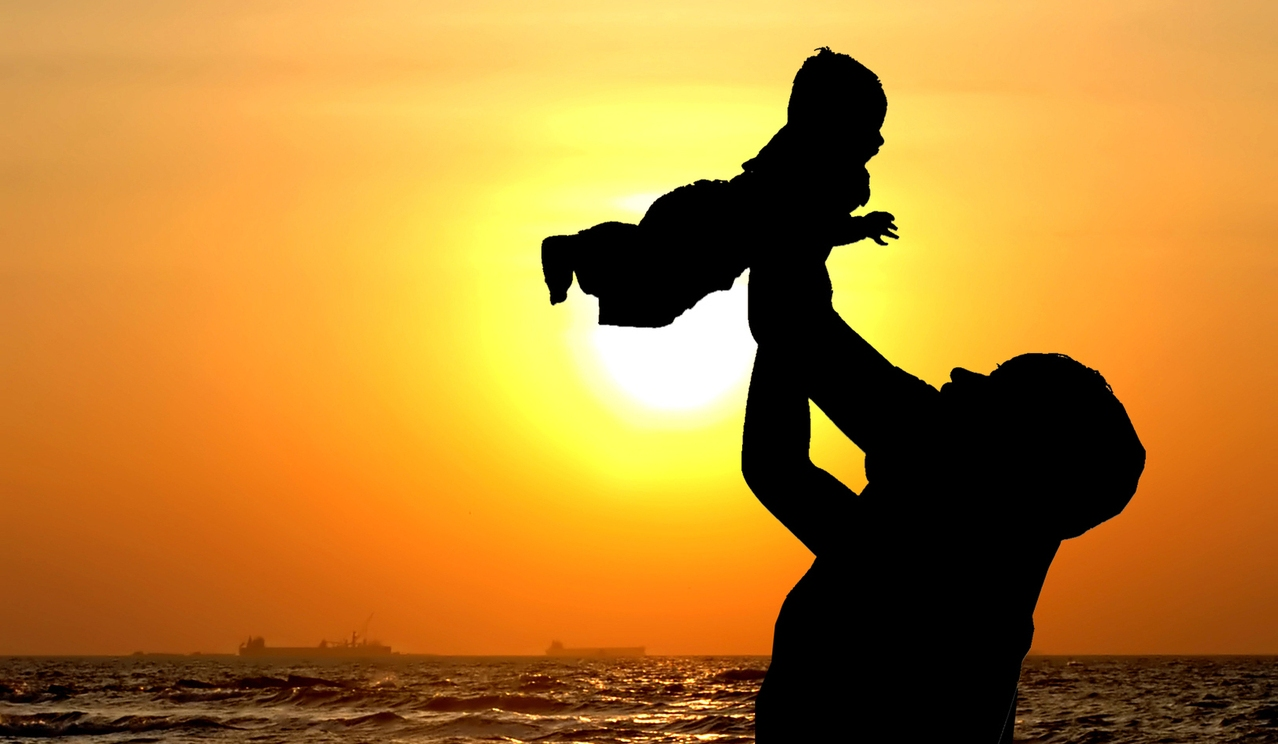
\includegraphics[width=0.4\textwidth]{ParentChild}}
            \end{itemize}
        \end{onlyenv}
        \begin{itemize}[<only@5->]
            \item In UNIX, processes are identified by a number called a PID (for Process IDentifier)
            \item Each \textbf{running} process has a unique identifier
            \item Do not assume anything about \PP{PIDs}: For all intents and purposes, they \PP{are random}!
            \item Each UNIX process also has a parent process which is the process that started it.
            \item The parent process can change to the \texttt{init} process if the parent process ends before the new process does \,$\to$\, i.e. \texttt{init} will pick up orphaned processes
        \end{itemize}
        \vspace{-2mm}
        \begin{varblock}{quote}[\textwidth]{System processes}[Greg's Wiki]<only@6-7>
            A process PID will \textbf{never} be freed up for use after the process dies until the parent process waits for the PID to see whether it ended and retrieve its exit code.
            If the parent ends, the process is returned to \textnormal{\texttt{init}}, which does this for you.
            This is important for one major reason: \alert{if the parent process manages its child process, it can be absolutely certain that, even if the child process dies, no other new process can accidentally recycle the child process PID until the parent process has waited for that PID and noticed the child died}.
            This gives the parent process the guarantee that the PID it has for the child process will \textbf{always} point to that child process, whether it is alive or a ``zombie''.
            Nobody else has that guarantee.
        \end{varblock}
        \begin{tikzpicture}[remember picture, overlay]
            \node[starburst, starburst point height=1cm, fill=yellow, draw=red, line width=2pt, visible on=<7>, rotate=10, font=\HUGE\bfseries, text=red, anchor=center] at ($(current page.center)-(0,22mm)$) {Not true in the shell!};
        \end{tikzpicture}
        \begin{onlyenv}<8>
            \vspace{-2mm}
            \begin{columns}[c]
                \begin{column}{0.25\textwidth}
                    \centering
\includegraphics[width=0.8\textwidth]{Danger}
                \end{column}
                \begin{column}{0.7\textwidth}
                    \begin{varblock}{quote}[\textwidth]{What happens in the shell}[Greg's Wiki]
                        Shells aggressively reap their child processes and store the exit status in memory, where it becomes available to your script upon calling \textnormal{\bash|wait|}.
                        But because the child might have already been reaped before you call wait, there is no zombie to hold the PID.\\
                        \alert{\textbf{The kernel is free to reuse that PID, and your guarantee has been violated!}}\\[-1.5ex] ~
                    \end{varblock}
                    \vspace{-3mm}
                    \centering\tiny We will see an explicit example in few slides
                \end{column}
            \end{columns}
        \end{onlyenv}
    \end{overlayarea}
    \PrepareURLsymbol[PB]
    \FrameRemark<2->{This article on \URL*{http://mywiki.wooledge.org/ProcessManagement}{Process Management} is good (long and advanced in its second part, though). Refer to it to discover more.}
\end{frame}
%~~~~~~~~~~~~~~~~~~~~~~~~~~~~~~~~~~~~~~~~~~~~%
\begin{frame}[fragile]{A bit of syntax: Retrieving a process PID}
    \vspace{-3mm}
    \begin{itemize}
        \item The \PB{\texttt{\$!}} special parameter holds the \PP{PID} of \textbf{the most recently executed background job}
              \begin{lstlisting}[style=MyBash, numbers=none, aboveskip=2mm, belowskip=-5mm, xrightmargin=25mm]
                  #!/bin/bash

                  #...
                  command &
                  pid=$!
                  # ...
              \end{lstlisting}
        \item You cannot reliably determine when or how a process was started purely from its identifier number (PID): \PP{do not make any assumption!}
        \item As you might know, there are some metadata stored together with the PID, such as the \textbf{process name} and the \textbf{issued command} to start the process. \alert{\textbf{Never rely on those!}}
    \end{itemize}
    \vspace{-1mm}
    \begin{varblock}{alert}[\textwidth]{Stay away from parsing the process tree!}
        UNIX comes with a set of handy tools, among which is \bash|ps|.
        This is a very helpful utility that you can use from the command line to get an overview of what processes are running.\\
        \alert{However, \bash|ps| output is unpredictable, highly OS-dependent, and not built for parsing!\\\textbf{Do not parse it in shell scripts! Ever!}}
    \end{varblock}
\end{frame}
%~~~~~~~~~~~~~~~~~~~~~~~~~~~~~~~~~~~~~~~~~~~~%
\begin{frame}[fragile]{A bit of syntax: The \bash|wait| builtin}
    \vspace{-1mm}
    \begin{overlayarea}{\textwidth}{0.7\textheight}
        \begin{lstlisting}[style=MyBash, numbers=none, belowskip=-6mm]
            wait |+[-fn] [jobspec or pid ...]+|
        \end{lstlisting}
        \begin{itemize}
            \item \alert<3>{\bash|wait| waits until the child process specified by each process ID \texttt{pid} or job specification \texttt{jobspec} exits and return the exit status of the last command waited for}
            \item \alert<2>{If no arguments are given, all currently active child processes are waited for, and the return status is zero}
            \item \alert<4>{\bash|wait -n|$\;$ waits for a single job to terminate and returns its exit status}
            \item \alert<5>{If not an active child process of the shell is passed to \bash|wait|, the return status is \textbf{127}}
        \end{itemize}
        \vspace{-2mm}
        \begin{onlyenv}<1>
            \centerline{\rule{8cm}{0.5pt}}
            \begin{itemize}
                \small
                \item If a job specification is given, all processes in the job are waited for
                \item Supplying the \bash|-f| option, when job control is enabled, forces \bash|wait| to wait for each \texttt{pid} or \texttt{jobspec} to terminate before returning its status, instead of returning when it changes status
            \end{itemize}
        \end{onlyenv}
        \begin{onlyenv}<2>
            \begin{lstlisting}[style=MyBash, numbers=none, aboveskip=3mm]
                # In a Bash script
                date
                { sleep 1; exit 1; } & { sleep 3; exit 2; } &
                { sleep 5; exit 3; } & { sleep 7; exit 4; } &
                wait # All currently active child processes are waited for
                date
            \end{lstlisting}
            \begin{lstlisting}[style=MyBash, numbers=none, aboveskip=1mm]
                $ ./script-above.bash
                |+Wed  4 Sep 16:13:27 CEST 2019
                Wed  4 Sep 16:13:34 CEST 2019+|
            \end{lstlisting}
        \end{onlyenv}
        \begin{onlyenv}<3>
            \begin{lstlisting}[style=MyBash, numbers=none, aboveskip=3mm]
                # In a Bash script
                date; sleep 3 & pid=$!
                echo "PID=${pid}";  ps -p ${pid};  wait ${pid}; date
            \end{lstlisting}
            \begin{lstlisting}[style=MyBash, numbers=none, aboveskip=1mm]
                $ ./script-above.bash
                |+Wed  4 Sep 16:17:19 CEST 2019
                PID=11353
                  PID TTY          TIME CMD
                11353 pts/11   00:00:00 sleep
                Wed  4 Sep 16:17:22 CEST 2019+|
            \end{lstlisting}
        \end{onlyenv}
        \begin{onlyenv}<4>
            \begin{lstlisting}[style=MyBash, numbers=none, aboveskip=3mm]
                # In a Bash script (-n option since Bash v4.3)
                { sleep 1; exit 1; } & { sleep 3; exit 2; } &
                { sleep 2; exit 3; } &
                for f in {1..3}; do
                   wait -n; echo "wait return status: $? at $(date +'%X')"
                done
            \end{lstlisting}
            \begin{lstlisting}[style=MyBash, numbers=none, aboveskip=1mm]
                $ ./script-above.bash
                |+wait return status: 1 at 16:36:16
                wait return status: 3 at 16:36:17
                wait return status: 2 at 16:36:18+|
            \end{lstlisting}
        \end{onlyenv}
        \begin{onlyenv}<5>
            \begin{lstlisting}[style=MyBash, numbers=none, aboveskip=3mm]
                $ wait 1234
                |+bash: wait: pid 1234 is not a child of this shell+|
                $ echo $?
                |+127+|
            \end{lstlisting}
        \end{onlyenv}
    \end{overlayarea}
\end{frame}
%~~~~~~~~~~~~~~~~~~~~~~~~~~~~~~~~~~~~~~~~~~~~%
\begin{frame}[fragile]{A bit of syntax: The \bash|kill| builtin}
    \vspace{-1mm}
    \begin{overlayarea}{\textwidth}{0.7\textheight}
        \begin{lstlisting}[style=MyBash, numbers=none, belowskip=-6mm]
            kill |+[-s sigspec] [-n signum] [-sigspec] jobspec or pid+|
        \end{lstlisting}
        \begin{itemize}
            \item Despite its name, the \bash|kill| command sends a signal to a process
            \item There are different way to specify a signal, use what you prefer
            \item If no signal is specified, SIGTERM (15) is sent
        \end{itemize}
        \begin{onlyenv}<1>
            \begin{lstlisting}[style=MyBash, style=smaller, numbers=none, xleftmargin=1mm]
                $ kill -l
                |+ 1) SIGHUP       2) SIGINT       3) SIGQUIT      4) SIGILL       5) SIGTRAP
                 6) SIGABRT      7) SIGBUS       8) SIGFPE       9) SIGKILL     10) SIGUSR1
                11) SIGSEGV     12) SIGUSR2     13) SIGPIPE     14) SIGALRM     15) SIGTERM
                16) SIGSTKFLT   17) SIGCHLD     18) SIGCONT     19) SIGSTOP     20) SIGTSTP
                21) SIGTTIN     22) SIGTTOU     23) SIGURG      24) SIGXCPU     25) SIGXFSZ
                26) SIGVTALRM   27) SIGPROF     28) SIGWINCH    29) SIGIO       30) SIGPWR
                31) SIGSYS      34) SIGRTMIN    35) SIGRTMIN+1  36) SIGRTMIN+2  37) SIGRTMIN+3
                38) SIGRTMIN+4  39) SIGRTMIN+5  40) SIGRTMIN+6  41) SIGRTMIN+7  42) SIGRTMIN+8
                43) SIGRTMIN+9  44) SIGRTMIN+10 45) SIGRTMIN+11 46) SIGRTMIN+12 47) SIGRTMIN+13
                48) SIGRTMIN+14 49) SIGRTMIN+15 50) SIGRTMAX-14 51) SIGRTMAX-13 52) SIGRTMAX-12
                53) SIGRTMAX-11 54) SIGRTMAX-10 55) SIGRTMAX-9  56) SIGRTMAX-8  57) SIGRTMAX-7
                58) SIGRTMAX-6  59) SIGRTMAX-5  60) SIGRTMAX-4  61) SIGRTMAX-3  62) SIGRTMAX-2
                63) SIGRTMAX-1  64) SIGRTMAX+|
                $ kill -l 15
                |+TERM+|
            \end{lstlisting}
        \end{onlyenv}
        \vspace{-2mm}
        \begin{varblock}{quote}[0.8\textwidth]{\bash|man 2 kill|}<only@2>
            If signal is 0, then no signal is sent, but existence and permission checks are still performed; this can be used to check for the existence of a process ID or process group ID that the caller is permitted to signal.
        \end{varblock}
        \begin{onlyenv}<2>
            \begin{lstlisting}[style=MyBash, aboveskip=2mm]
                # Waiting for a process to end
                # (when you have permissions to send signals)
                while kill -0 "${pid}"; do
                    sleep 1
                done
            \end{lstlisting}
        \end{onlyenv}
    \end{overlayarea}
    \FrameRemark{The \bash|kill| builtin offers more complex functionalities, like sending a signal to a process group when the used PID is negative. Read about it in the manual.}
\end{frame}
%~~~~~~~~~~~~~~~~~~~~~~~~~~~~~~~~~~~~~~~~~~~~%
\begin{frame}[fragile]{A potentially catastrophic hidden danger}
    \begin{overlayarea}{\textwidth}{0.5\textheight}
        \begin{onlyenv}<2-4>
            \begin{lstlisting}[style=MyBash]
                #!/bin/bash
                                            #  EXAMPLE 1: wait
                ( exit 12 ) &
                pid=$!
                while { sleep 0 & [[ "${pid}" |+!=+| "$!" ]]; }; do
                    :
                done
                wait "$pid"
                echo "$?"
            \end{lstlisting}
        \end{onlyenv}
        \begin{onlyenv}<5>
            \begin{lstlisting}[style=MyBash, emph={[8]long_running_command}, firstnumber=10]
                #!/bin/bash
                                            #  EXAMPLE 2: kill
                long_running_command &
                pid=$!
                echo "Killing long_running_command on PID ${pid} in 24h"
                sleep 86400
                echo 'Time up!'
                kill "${pid}"
            \end{lstlisting}
            \begin{center}
                \Large \PQ{Who will receive the SIGTERM signal?!}
            \end{center}
        \end{onlyenv}
        \begin{uncoverenv}<3-4>
            \begin{lstlisting}[style=MyBash, numbers=none, aboveskip=1mm]
                $ ./script-above.bash
                |+0+|   # Yes, 0 and not 12... WHAAAAAT?
            \end{lstlisting}
        \end{uncoverenv}
        \begin{center}
            \only<2>{
\includegraphics[width=3cm]{MemeEatingCereals}}
            \only<3>{
\includegraphics[width=4cm]{MemeSplitting}}
        \end{center}
    \end{overlayarea}
    \begin{varblock}{alert}[0.9\textwidth]{\textbf{Sad but true!}}<only@4->
        The way shells are programmed, as soon as a child process dies, the shell will call \PB{\emph{wait()}} on it right away (storing the termination status as part of its internal state), which will free the PID for reuse by another process.
    \end{varblock}
\end{frame}
%~~~~~~~~~~~~~~~~~~~~~~~~~~~~~~~~~~~~~~~~~~~~%
\begin{frame}[fragile]{I absolutely need to know if the PID is the right one, what should I do?}
    \vspace{-3mm}
    \large
    \begin{varblock}{example}[\textwidth]{\textbf{Do not use Bash!}}<2->
        Yes, implement the code launching a background process in C or Python, Perl, Ruby, etc.
        \textbf{Not in shell.}
        Those will not have this problem, since they won't reap children by default (like the shell does) and you will have to do it explicitly there.
        Or consider launching background processes using a system manager, such as \bash|systemd|.
    \end{varblock}
    \small
    \begin{varblock}{}[0.95\textwidth]{However}<only@3>
        Note that the kernel will typically try hard to avoid reusing PIDs, at least try to delay reusing a PID, exactly because in some cases there are no guarantees that the PID hasn't been reused, so the kernel tries to minimise this situation where a signal will be delivered to the wrong process.
    \end{varblock}
    \vspace{-2pt}
    \begin{onlyenv}<4>
        \begin{varblock}{}[0.95\textwidth]{Alternatively}
            You can save the start time of the original process and, before using it, check that the start time of the process with that PID matches what you saved.
            The pair PID, start-time is a unique identifier for the processes in Linux.
            However, this does not solve the issue here.
        \end{varblock}
        \begin{lstlisting}[style=MyBash, numbers=none]
            $ sleep 10 &
            |+[1] 4451+|
            $ ps -p 4451 -h -o lstart
            |+Thu Sep  5 18:22:43 2019+|
        \end{lstlisting}
    \end{onlyenv}
\end{frame}
%~~~~~~~~~~~~~~~~~~~~~~~~~~~~~~~~~~~~~~~~~~~~%
\begin{frame}[fragile]{A work-around for exit codes}
    \vspace{-1mm}
    \begin{overlayarea}{\textwidth}{\textheight}
        \begin{itemize}
            \item If you have several (maybe long) processes in background during the execution of a script and you are interested in their exit code, you can write them to a file
            \item Alternatively, a possible idea is to use redirection faking a file and taking advantage of the fact that \PP{\textbf{in Bash the processes inside the process substitution are not waited for}}
        \end{itemize}
        \begin{onlyenv}<1>
            \begin{lstlisting}[style=MyBash, aboveskip=3mm, emph={[7]command_pid, exitCode}, emph={[8]another_command}]
                #!/bin/bash
                {
                    command_pid=$!
                    # ...
                    another_command &
                    # ...
                    read <&3 exitCode
                    if [[ "${exitCode}" -eq 0 ]]; then
                        echo "command was successful!"
                    fi
                } 3< <(command > logfile 2>&1; echo "$?")
            \end{lstlisting}
        \end{onlyenv}
        \begin{onlyenv}<2-3>
            \begin{lstlisting}[style=MyBash, aboveskip=3mm, emph={[7]sleep_pid, exitCode, waitCode}, firstnumber=12, xrightmargin=2mm]
                #!/bin/bash
                {
                    sleep_pid=$!
                    while { ( exit 12 ) & [[ "${sleep_pid}" |+!=+| "$!" ]]; }; do
                        :
                    done
                    wait "${sleep_pid}"
                    waitCode=$?
                    read <&3 exitCode
                    echo "Command in process substitution: ${exitCode}"
                    echo "Command in           while loop: ${waitCode}"
                } 3< <(sleep 1; echo "$?")
            \end{lstlisting}
            \begin{uncoverenv}<3>
                \begin{lstlisting}[style=MyBash, numbers=none, aboveskip=1mm, xrightmargin=2mm]
                    $ ./script-above.bash
                    |+Command in process substitution: 0
                    Command in           while loop: 12+|
                \end{lstlisting}
            \end{uncoverenv}
        \end{onlyenv}
    \end{overlayarea}
\end{frame}
%~~~~~~~~~~~~~~~~~~~~~~~~~~~~~~~~~~~~~~~~~~~~%
\begin{frame}{Process Management: Conclusions}
    \vspace{-2mm}
    \begin{overlayarea}{\textwidth}{0.7\textheight}
        \begin{itemize}[<only@1-2>]
            \setlength{\itemsep}{0mm}
            \item It is a potentially tough world: Be scared but not too much
            \item Bash might not be the most appropriate tool
            \item Be aware of the truth (what we just discussed)
            \item If you want to have something running in background, why do you want so?
            \item There are tools which you might consider:\\[0.3ex]
            \begin{enumerate}
                \item \bash|systemd| (system manager)
                \item \bash|timeout| (run a command with a time limit)
                \item \bash|xargs -P| \,or\, \bash|parallel| (to run independent tasks in parallel)
            \end{enumerate}
        \end{itemize}
        \begin{varblock}{quote}[\textwidth]{About using $\;$\bash|kill -9|}[Greg's Wiki]<only@2>
            Do not use kill -9, ever.
            For any reason.
            \textbf{Unless you wrote the program to which you're sending the SIGKILL, and know that you can clean up the mess it leaves.}
            Because you're debugging it.
            If a process is not responding to normal signals, it's probably in ``state D'' (as shown on \textnormal{\bash|ps u|}), which means it's currently executing a system call.
            If that's the case, you're probably looking at a dead hard drive, or a dead NFS server, or a kernel bug, or something else along those lines.\\
            And you won't be able to kill the process anyway, SIGKILL or not.
        \end{varblock}
    \end{overlayarea}
    \begin{tikzpicture}[remember picture, overlay, scope on=<3>, every node/.style={inner sep=0mm}]
        \node[left  = 1mm of current page.center, yshift=-2mm] {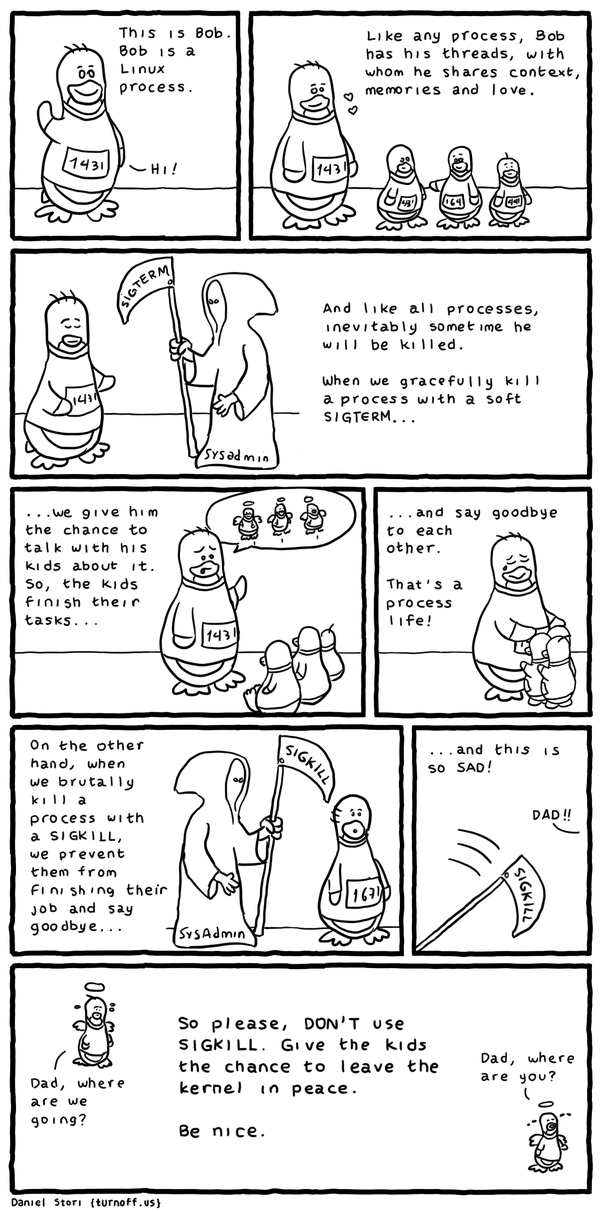
\includegraphics[width=56mm, clip, trim=0 173mm 0 0]{Sigkill}};
        \node[right = 1mm of current page.center, yshift=-2mm] {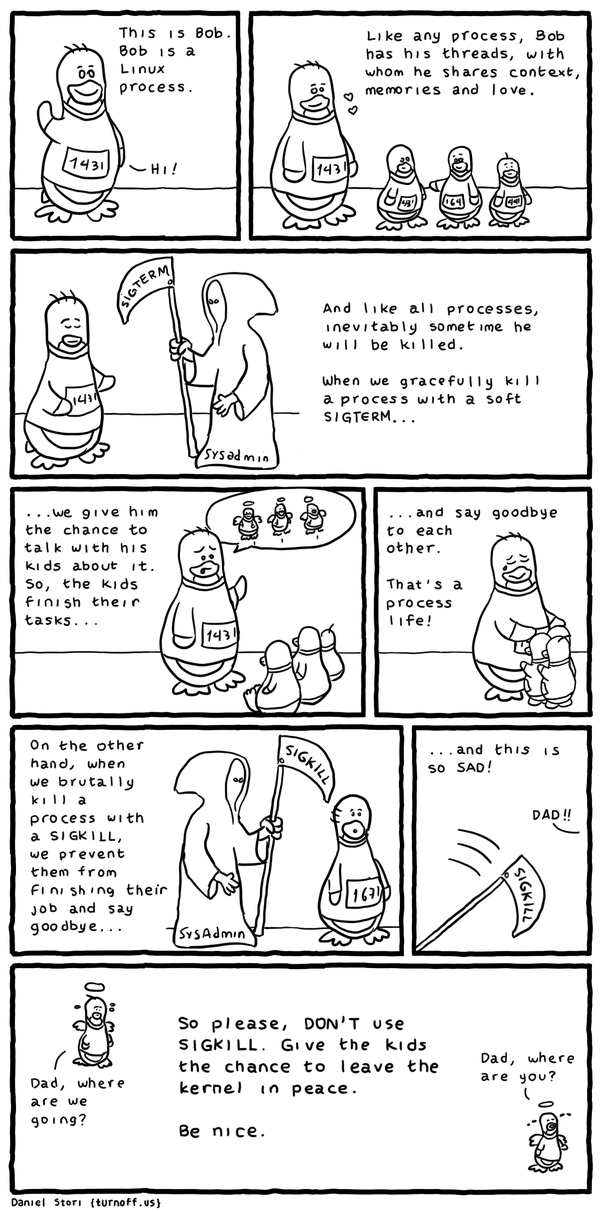
\includegraphics[width=56mm, clip, trim=0 0 0 255mm]{Sigkill}};
    \end{tikzpicture}
\end{frame}







    \addSection{Traps}[0.5,0.5]{example-image-b}{image}
    %-------------------------------%
%  Author: Alessandro Sciarra   %
%    Date: 6 Sep 2019           %
%-------------------------------%

%~~~~~~~~~~~~~~~~~~~~~~~~~~~~~~~~~~~~~~~~~~~~%
\begin{frame}[fragile]{Motivation}
    \vspace{-2mm}
    Consider the following script (\alert{not nice code}):
    \begin{lstlisting}[style=MyBash, aboveskip=3mm, belowskip=-5mm]
        #!/usr/bin/env bash

        function CreateAuxiliaryFiles(){
            # ...
        }
        function CleanAuxiliaryFiles(){
            # ...
        }
        CreateAuxiliaryFiles
        gnuplot "${temporaryFileToPlot}"
        if [[ "${savePlot}" = 'TRUE' ]]; then
            pdflatex "${outputFilename}.tex"
        fi
        CleanAuxiliaryFiles
        exit 0
    \end{lstlisting}
    \begin{varblock}{alert}[\textwidth]{}
        \Large \alert{What happens if the script is terminated by the user, e.g. via CTRL-C?}
    \end{varblock}
\end{frame}
%~~~~~~~~~~~~~~~~~~~~~~~~~~~~~~~~~~~~~~~~~~~~%
\begin{frame}{Signal handlers or traps}
    \begin{onlyenv}<1-2>
        \begin{itemize}
            \item As you know you can send signals to processes via the \bash|kill| builtin
            \item However, in shell scripts, \PP{\textbf{it is possible to associate a behaviour upon receiving a signal!}}
            \item If you think about it, it is a very powerful technique
            \item In order to perform an action when a signal is received, a trap has to be set up
        \end{itemize}
        \smallskip
        \begin{center}
            \begin{tikzpicture}
                \begin{scope}[every node/.style={thick, ellipse, minimum width=2cm}]
                    \node[draw=PB, fill=PP!20] (a) {Process A};
                    \node[draw=PQ, fill=PT!20, below right = of a] (b) {Process B};
                \end{scope}
                \begin{scope}[scope on=<2>]
                    \path[to] (a) edge[out=0, in=90] node[midway, right=2mm, font=\small, text=PS] {Signal} (b);
                    \path[to] (b) edge[out=270, in=180] node[pos=1, right=1mm] {Do the action associated to the signal} ++(1cm, -15mm);
                    \node[right = 0mm of b] {\Remark{Process B traps the signal}};
                \end{scope}
            \end{tikzpicture}
        \end{center}
    \end{onlyenv}
    \begin{onlyenv}<3>
        \medskip
        \colorbox{background-color}{\bash|trap 'some code' signal(s)|}\\[0.3em]
        \begingroup\leftskip1em
            Using this form, a signal handler is set up for each signal in the list\\
            When one of these signals is received, the commands in the first argument will be executed\\[0.4em]
        \endgroup
        \colorbox{background-color}{\bash|trap '' signal(s)|}\\[0.3em]
        \begingroup\leftskip1em
            Using this form, each signal in the list will be ignored. \alert{Most scripts should not do this!}\\[0.4em]
        \endgroup
        \colorbox{background-color}{\bash|trap - signal(s)|}\\[0.3em]
        \begingroup\leftskip1em
            Using this form, each signal in the list will be restored to its default behaviour\\[0.4em]
        \endgroup
        \colorbox{background-color}{\bash|trap signal|}\\[0.3em]
        \begingroup\leftskip1em
            Legacy syntax: As the previous but for one signal only!\Remark{Prefer the previous, slightly more explicit syntax}\\[0.4em]
        \endgroup
        \colorbox{background-color}{\bash|trap|}\\[0.3em]
        \begingroup\leftskip1em
            With no arguments, print a list of signal handlers\\
        \endgroup
    \end{onlyenv}
\end{frame}
%~~~~~~~~~~~~~~~~~~~~~~~~~~~~~~~~~~~~~~~~~~~~%
\begin{frame}{Common used signals}
    \begin{description}[TERMX]
        \item[\textbf{HUP}] Hang Up. The controlling terminal has gone away.
        \item[\textbf{INT}] Interrupt. The user has pressed the interrupt key (usually \textbf{Ctrl-C} or \textbf{DEL}).
        \item[\textbf{QUIT}] Quit. The user has pressed the quit key (usually \textbf{Ctrl-\textbackslash}). Exit and dump core.
        \item[\textbf{KILL}] Kill. \alert{This signal cannot be caught or ignored.} Unconditionally fatal. \textbf{\textbf{No cleanup possible.}}
        \item[\textbf{TERM}] Terminate. This is the default signal sent by the \bash|kill| builtin.
        \item[\textbf{EXIT}] Not really a signal. In a Bash script (non-interactive), an EXIT trap is run on any exit, signalled or not. In other POSIX shells only when the shell process exits.
    \end{description}
    \begin{varblock}{}[0.9\textwidth]{Remember}
        If you are asking a program to terminate, you should always use SIGTERM. % (simply \bash|kill process_ID|).
        This will give the program a chance to catch the signal and clean up.
        If you use SIGKILL, the program cannot clean up, and \textbf{may leave files in a corrupted state}.
    \end{varblock}
\end{frame}
%~~~~~~~~~~~~~~~~~~~~~~~~~~~~~~~~~~~~~~~~~~~~%
\begin{frame}[fragile]{A simple example}
    \vspace{-4mm}
    \begin{varblock}{quote}[\textwidth]{Common use case}
        \normalsize\textnormal{Traps can be set up to intercept a fatal signal, perform cleanup, and then exit gracefully.}
    \end{varblock}
    \begin{lstlisting}[style=MyBash, emph={[7]temporaryFile}, belowskip=-5mm]
        #!/usr/bin/env bash

        temporaryFile=$(mktemp) || exit
        trap 'rm -f "${temporaryFile}"' EXIT
    \end{lstlisting}
    Use a function whenever you need to achieve a more complex task
    \begin{lstlisting}[style=MyBash, emph={[7]temporaryFile}, aboveskip=2mm, belowskip=-5mm, xleftmargin=2mm, xrightmargin=3mm, firstnumber=5]
        #!/usr/bin/env bash

        function CleanAuxiliaryFiles(){ # If you trap INT (CTRL-C)
            # ...                       # do not forget to exit unless
        }                               # you have reasons not to do so
        trap 'CleanAuxiliaryFiles' EXIT
    \end{lstlisting}
    \small
    \begin{varblock}{}[\textwidth]{Only in Bash!}
        The special name EXIT is preferred for any signal handler that simply wants to clean up upon exiting.
        So to clean up, just trap EXIT and call a cleanup function from there. \textbf{Don't trap a bunch of signals.}
    \end{varblock}
\end{frame}
%~~~~~~~~~~~~~~~~~~~~~~~~~~~~~~~~~~~~~~~~~~~~%
\begin{frame}[fragile]{When is the signal exactly handled?}
    \vspace{-5mm}
    \begin{varblock}{alert}[0.9\textwidth]{A subtle but important feature}
        When Bash is executing an external command in the foreground, it does not handle any signals received until the foreground process terminates.
    \end{varblock}
    \vspace{2mm}
    \begin{overlayarea}{\textwidth}{0.28\textheight}
        \begin{onlyenv}<1>
            \begin{lstlisting}[style=MyBash]
                #!/usr/bin/env bash

                echo "My PID is $$ and my PGID is $(ps -h -p $$ -o pgid)"
                trap 'echo "Doing some cleaning before exiting!"' EXIT
                echo "Wait 1h"
                sleep 3600
            \end{lstlisting}
        \end{onlyenv}
        \begin{onlyenv}<2>
            \begin{lstlisting}[style=MyBash, firstnumber=7]
                #!/usr/bin/env bash

                echo "My PID is $$ and my PGID is $(ps -h -p $$ -o pgid)"
                trap 'echo "Doing some cleaning before exiting!"' EXIT
                echo "Wait 1h"; sleep 3600 & wait $!
                # Note that sleep 3600 will not be killed and will
                # continue to run when you send a INT signal!
            \end{lstlisting}
        \end{onlyenv}
        \begin{onlyenv}<3>
            \begin{lstlisting}[style=MyBash, firstnumber=14]
                #!/usr/bin/env bash

                echo "My PID is $$ and my PGID is $(ps -h -p $$ -o pgid)"
                unset -v pid
                trap 'echo "Cleaning!"; [[ $pid ]] && kill "${pid}"' EXIT
                echo "Wait 1h"
                sleep 3600 & pid=$!; wait
            \end{lstlisting}
        \end{onlyenv}
    \end{overlayarea}
    \vspace{-1.5mm}
    \begin{itemize}
        \item If you kill the script using $\;$\bash|kill -s INT|$\;$ from another terminal (not with CTRL-C), bash will wait for \bash|sleep| to exit before calling the trap\\
              $\;\to\;$\alert{\textbf{That's probably not what you expect!}}
        \item<2-> A work-around is to use a \PB{\textbf{builtin}} that will be interrupted, such as \bash|wait|
        \item<2-> \PP{Any bash internal command will be interrupted by a (non-ignored) incoming signal!}
        \item<3-> If you want the background job to be killed when the script is killed, add that to the trap!
    \end{itemize}
\end{frame}
%~~~~~~~~~~~~~~~~~~~~~~~~~~~~~~~~~~~~~~~~~~~~%
\begin{frame}[fragile]{What indeed is CTRL-C doing?}
    \vspace{-3mm}
    Let us consider again the previous example
    \begin{lstlisting}[style=MyBash, numbers=none, aboveskip=2mm, belowskip=-4mm]
        #!/usr/bin/env bash

        echo "My PID is $$ and my PGID is $(ps -h -p $$ -o pgid)"
        trap 'echo "Doing some cleaning before exiting!"' EXIT
        echo "Wait 1h"; sleep 3600
    \end{lstlisting}
    \begin{overlayarea}{\textwidth}{0.5\textheight}
        \begin{itemize}
            \item<1-> As said, sending to this script the INT signal from another terminal does not terminate it
            \item<1-> However, CTRL-C does terminate it\ldots\ but why?
            \item<2-> Because \PP{\textbf{processes are organised in groups}}:
                      \begin{itemize}
                          \item The leader process (i.e. the process that created the group)
                          \item Any other process started by the leader process
                      \end{itemize}
            \item<2-> \alert{\textbf{CTRL-C sends the INT signal to the entire process group}}
            \item<2-> Terminals keep track of the foreground process group: When receiving a CTRL-C, they send the SIGINT to the entire foreground group!
        \end{itemize}
        \begin{onlyenv}<3>
            \begin{lstlisting}[style=MyBash, numbers=none, xleftmargin=2mm, xrightmargin=2mm]
                kill -s INT -123 # will kill the process group with the ID 123
            \end{lstlisting}
        \end{onlyenv}
    \end{overlayarea}
    \FrameRemark{Note that you can't rely on the process group ID of a script to be the same as \texttt{\$\$}, as that depends greatly on how the script was started.}
\end{frame}
%~~~~~~~~~~~~~~~~~~~~~~~~~~~~~~~~~~~~~~~~~~~~%
\begin{frame}[fragile]{Trapping SIGINT and SIGQUIT: Be careful!}
    \vspace{-1mm}
    \begin{overlayarea}{\textwidth}{0.7\textheight}
        \begin{itemize}
            \item Bash is among a few shells that implement a \textbf{wait and cooperative exit} approach at handling SIGINT/SIGQUIT delivery
            \item When interpreting a script, upon receiving a SIGINT,
            \begin{enumerate}
                \item \textbf{it doesn't exit straight away}, instead
                \item \PP{it waits for the currently running command to return} and
                \item \alert{it only exits -- \textbf{by killing itself with SIGINT} -- if that command was also killed by that SIGINT}
            \end{enumerate}
            \item<only@1> The idea is that, if your script calls \bash|vi| for instance, and you press CTRL-C within \bash|vi| to cancel an action, that should not be considered as a request to abort the script
        \end{itemize}
        \begin{varblock}{alert}[0.9\textwidth]{What does it mean?}<only@1>
            Imagine you're writing a script and that script exits normally upon receiving SIGINT.
            That means that if that script is invoked from another bash script, \\\alert{\textbf{CTRL-C will no longer interrupt that other script!}}
        \end{varblock}
        \begin{onlyenv}<2>
            \begin{varblock}{}[0.95\textwidth]{}
                \small The \bash|ping| command returns with 0 when host is reachable (the ping has been answered) and non-zero otherwise when interrupted (which is the only way for ping to return in that case).
            \end{varblock}
            \begin{lstlisting}[style=MyBash, aboveskip=0mm, belowskip=-6mm]
                #!/usr/bin/env bash
                for index in {1..254}; do
                    ping -c 2 "192.168.1.${index}"
                done
            \end{lstlisting}
            \begin{varblock}{}[0.95\textwidth]{}
                \small CTRL-C will send a INT signal to the script, but since \bash|ping| just returns 0 or 1 and is not killed by SIGINT, only the \alert{\textbf{current}} \bash|ping| will terminate and the \bash|for| loop will continue!
            \end{varblock}
        \end{onlyenv}
        \begin{onlyenv}<3>
            \begin{varblock}{}[1.03\textwidth]{}
                Commands that don't have a SIGINT handler (like \bash|sleep|) or \textbf{do the right thing of killing themselves with SIGINT upon receiving SIGINT} (like \bash|bash| itself does) don't exhibit the problem!
            \end{varblock}
            \begin{lstlisting}[style=MyBash, firstnumber=5]
                #!/usr/bin/env bash
                index=1
                while [[ "${index}" -le 100 ]]; do
                  printf "%d " "$((index++))"
                  sleep 1
                done; echo  # This script terminates correctly via CTRL-C
            \end{lstlisting}
        \end{onlyenv}
        \begin{onlyenv}<4>
            \medskip
            \begin{varblock}{alert}[\textwidth]{\large Take-home lesson}
                If you choose to set up a handler for SIGINT (rather than using the EXIT trap), you should be aware that \alert{\textbf{a process that exits in response to SIGINT should kill itself with SIGINT rather than simply exiting}}, to avoid causing problems for its caller.
                The same goes for SIGQUIT.
            \end{varblock}
            \begin{lstlisting}[style=MyBash, numbers=none]
                trap 'DoYourStuffHere; trap - INT; kill -s INT "$$"' INT
            \end{lstlisting}
        \end{onlyenv}
    \end{overlayarea}
\end{frame}












    \addSection{Awk and Sed}[0.5,0.5]{example-image-b}{image}
    %-------------------------------%
%  Author: Alessandro Sciarra   %
%    Date: 10 Sep 2019          %
%-------------------------------%

%~~~~~~~~~~~~~~~~~~~~~~~~~~~~~~~~~~~~~~~~~~~~%
\begin{frame}{Why do we need them?}
    \vspace{-3mm}
    \begin{itemize}
        \item In science, most of our time in the terminal is spent acting on files
        \item Mastering file handling in general can allow us to simplify the data analysis software
        \item Typical operations might be
              \begin{itemize}
                  \item Prepare data for plotting in a given format
                  \item Search patterns in a file
                  \item Extract portion of a file
                  \item Transform a file (e.g. remove trailing spaces)
                  \item \ldots
              \end{itemize}
    \end{itemize}
    \begin{varblock}{}[0.95\textwidth]{GNU Core Utilities}
        \begin{tabular}{*{7}{>{\ttfamily\color{external-color}}c}}
            head    &  cat    &  sum     &  column  &  sort   &  join  &  expand   \\
            tail    &  tac    &  cksum   &  paste   &  uniq   &  comm  &  unexpand \\
                    &  cut    &  md5sum  &          &         &  tr    &  split    \\
        \end{tabular}
    \end{varblock}
    \begin{tikzpicture}[remember picture, overlay]
        \coordinate (C) at ($(current page.center)!0.5!(current page.south)$);
        \begin{scope}[every node/.style={starburst, starburst point height=6mm, fill=yellow, draw=red, ultra thick, text=red, font=\Huge\ttfamily, visible on=<2>, rotate=10}]
            \node[left  = of C, yshift=5mm] {sed};
            \node[right = of C, yshift=1mm] {awk};
        \end{scope}
        \node[anchor=east, visible on=<2>] at ($(current page.east)+(-6mm,6mm)$) {
\includegraphics[width=32mm, clip, trim=1mm 3mm 1mm 48mm]{InfinitePower}};
    \end{tikzpicture}
    \FrameRemark{A complete \URL[PB]{https://en.wikipedia.org/wiki/List\_of\_GNU\_Core\_Utilities\_commands}{GNU coreutils list} is available on Wikipedia.}
\end{frame}
%~~~~~~~~~~~~~~~~~~~~~~~~~~~~~~~~~~~~~~~~~~~~%






    %------------3mm-------------------%
%  Author: Alessandro Sciarra   %
%    Date: 10 Sep 2019          %
%-------------------------------%

%~~~~~~~~~~~~~~~~~~~~~~~~~~~~~~~~~~~~~~~~~~~~%
\makeatletter
\@ifundefined{tmpbox}{%
    \newsavebox{\tmpbox}%
}{}
\makeatother
%~~~~~~~~~~~~~~~~~~~~~~~~~~~~~~~~~~~~~~~~~~~~%
\begin{frame}{Sed: A marvellous utility}
    \vspace{-3mm}
    \begin{varblock}{quote}[\textwidth]{The awful truth about \bash|sed|}
        \textnormal{Sed is extremely powerful.
        Unfortunately, most people never learn its real power.
        The language is simpler than the average user thinks, because the documentation is far from being ideal.
        Sed has several commands, but most people only learn the substitute command \texttt{'s'}.
        And the GNU manual begins exactly with examples about the \texttt{'s'} command.}
    \end{varblock}
    \vspace{-1mm}
    \PrepareURLsymbol[PB]
    \begin{varblock}{example}[\textwidth]{Not bad!}
        The substitute command is just one command.
        Sed has at least 20 different commands for you.
        You can even write \URL*{https://catonmat.net/wp-content/uploads/2008/09/sedtris.sed}{Tetris} in it (not to mention that \PS{it's Turing complete}).
    \end{varblock}
    \vspace{-1mm}
    \begin{lrbox}{\tmpbox}
        \begin{minipage}{0.75\textwidth}
            \URL[PB]{https://www.gnu.org/software/sed/manual}{The official GNU manual} \Remark{The PDF is 85 pages long\ldots}\\
            \URL[PS]{http://www.grymoire.com/Unix/Sed.html}{A very nice tutorial} \Remark{Bash code there often uses deprecated features, but you should know it by now!}\\
            \URL[PT]{http://sed.sourceforge.net/sed1line.txt}{One-liners, with some comments}\\
            \URL[PQ]{https://catonmat.net/sed-one-liners-explained-part-one}{More one-liners, explained but advanced!}
        \end{minipage}
    \end{lrbox}
    \begin{varblock*}{}[0.76\textwidth]{Some references}
        \usebox{\tmpbox}
    \end{varblock*}
\end{frame}
%~~~~~~~~~~~~~~~~~~~~~~~~~~~~~~~~~~~~~~~~~~~~%
\begin{frame}[fragile]{The PDF manual is 85 pages long. What should I learn here?}
    \vspace{-4mm}
    \begin{itemize}
        \item We will focus on the abstract idea of \textbf{how} \bash|sed| processes a file
        \item Some of the simplest commands (acting on a single line) will be introduced
        \item Learning Sed is almost like learning a new programming language, mastering it is probably not needed for a physicist either
    \end{itemize}
    \begin{uncoverenv}<2->
        \begin{lstlisting}[style=MyBash, numbers=none, aboveskip=2mm, belowskip=-5mm]
            # Invocation
            sed |+[OPTIONS...] [SCRIPT] [INPUTFILE...]+|

            # General command syntax to be put in [SCRIPT]
            [addr]X[options]
        \end{lstlisting}
    \end{uncoverenv}
    \begin{itemize}[<3>]
        \item \texttt{X} is a \bash|sed| command
        \item \texttt{[addr]} is an optional line address\\
              If \texttt{[addr]} is specified, the command \texttt{X} will be executed only on the matched lines;\\
              \texttt{[addr]} can be a single line number, a regular expression, or a range of lines
        \item Additional \texttt{[options]} are used for some \bash|sed| commands
        \item Quote the commands to avoid shell globbing conflicts\\
              $\to$ usually you want to use single quotes
    \end{itemize}
\end{frame}
%~~~~~~~~~~~~~~~~~~~~~~~~~~~~~~~~~~~~~~~~~~~~%
\begin{frame}{Some of the most used commands}
    \vspace{-2mm}
    \begin{description}[XXX]
        \item[{s/regexp/replacement/[flags]}] ~\\[0.5ex]
            Match the regular-expression against the content of the pattern space.\\
            If found, replace matched string with replacement.
        \item[p] ~\\[0.5ex]
            Print the pattern space, up to the first newline.
        \item[d] ~\\[0.5ex]
            Delete the pattern space; immediately start next cycle.
        \item[=] ~\\[0.5ex]
            Print the current input line number (with a trailing newline).
        \item[\{ cmd ; cmd \ldots \}] ~\\[0.5ex]
            Group several commands together.
        \item[q] ~\\[0.5ex]
            Exit \bash|sed| without processing any more commands or input.
    \end{description}
\end{frame}
%~~~~~~~~~~~~~~~~~~~~~~~~~~~~~~~~~~~~~~~~~~~~%
\begin{frame}{A \bash|sed| cycle: Being line oriented}
    \vspace{-1mm}
    \begin{overlayarea}{\textwidth}{0.26\textheight}
        \begin{enumerate}
            \setcounter{enumi}{-1}
            \item<only@0> % Here I cheat and I do a horrible work-around to avoid a vertical shift I have no clue why it occurs!
            \item<only@2> The next line is read from the input file and placed it in the pattern space.\\
                          If the end of file is found, and if there are additional files to read, the current file is closed, the next file is opened, and the first line of the new file is placed into the pattern space.
            \item<only@3> The line count is incremented by one.\\
                          Opening a new file does not reset this number.
            \item<only@4> Each \bash|sed| command is examined.
                          If there is a restriction placed on the command, and the current line in the pattern space meets that restriction, the command is executed.
                          Some commands, like \texttt{'d'} cause \bash|sed| to go to the top of the loop.
                          The \texttt{'q'} command causes \bash|sed| to stop.
                          Otherwise the next command is examined.
            \item<only@5> After all of the commands are examined, the pattern space is printed to the output (unless sed has the optional "-n" argument) and the pattern space is emptied.
        \end{enumerate}%}
    \end{overlayarea}
    \begin{center}
        \begin{tikzpicture}
            \coordinate (O) at (0,0);
            \begin{scope}[node distance=4mm, every node/.style={thick}]
                \node[draw=PB, background fill=PP!10,  fill on=<2-4>, cloud, cloud puffs=11, text=PB, text width=1cm, align=center] (space) at (O) {Pattern space};
                \node[draw, fill=gray!20, ellipse, above = of space, xshift=55mm] (file) {Input file};
                \node[draw=PS, fill=PS!10, ellipse, text=PS, below = of space, xshift=55mm] (output) {Output};
                \node[draw=PQ, fill=PT!10, circle, text=PQ, above = of space, xshift=-35mm, label=below:{\footnotesize Line counter}] (linenr) {=\strut};
                \node[draw=PB, fill=PB!20, rounded corners=1mm, text=black, below = of space, xshift=-25mm] (exit) {EXIT};
            \end{scope}
            \path[to, visible on=<2->] (file) edge[out=180, in=90, looseness=0.6] node[pos=0.3, above=2pt, font=\scriptsize] {Read line into pattern space} (space);
            \path[to, visible on=<3->, overlay] (linenr) edge[out=60, in=330, looseness=4] node[pos=0.5, right, font=\scriptsize\ttfamily, text=PQ] {++} (linenr);
            \path[to, visible on=<4->] (space) edge[out=60, in=330, looseness=3] node[pos=0.5, right, font=\scriptsize, text=PP] {Every command is examined and maybe executed} (space)
                                               edge[out=300, in=150, looseness=0.6] node[pos=0.6, above, font=\scriptsize, text=PS] {Some commands print something} (output)
                                               edge[out=180, in=90] node[pos=0.4, left=2mm, font=\scriptsize, text=PB] {Sed might terminate} (exit);
            \path[to, visible on=<5->] (space) edge[out=270, in=180, looseness=0.6] node[pos=0.6, below=1mm, font=\scriptsize, text=PS] {Print, maybe, and empty pattern space} (output);
        \end{tikzpicture}
    \end{center}
    \FrameRemark{There is also a hold space and this flow gets modified by more complex commands. This is a good approximation.}
\end{frame}
%~~~~~~~~~~~~~~~~~~~~~~~~~~~~~~~~~~~~~~~~~~~~%
\begin{frame}[fragile]{Address restrictions}
    \vspace{-3mm}
    \begin{varblock}{quote}[\textwidth]{A command can be limited to some lines using restrictions}
        \vspace{-2mm}\textnormal{
            \begin{itemize}
                \item A positive line number (use \texttt{\$} to refer to the last line)
                \item A regular expression \PP{\texttt{/regex/}} or \PP{\texttt{\textbackslash$\bullet$regex$\bullet$}} where \PP{$\bullet$} is any character \Remark{not to be matched!}
                \item Use an exclamation mark after the address to negate that address
                \item A comma separated pair to specify a range of lines
            \end{itemize}
        }
    \end{varblock}
    \begin{lstlisting}[style=MyBash, numbers=none]
        |++|                # Command applies
        |+3+|               #  - to line 3 only
        |+/^#/+|            #  - to lines starting by #
        |+\%^//%+|          #  - to lines starting by //
        |+5!+|              #  - not to line 5
        |+1,3+|             #  - to first three lines
        |+3,$+|             #  - from line 3 to the end
        |+1,/one/+|         #  - till the first line matching 'one'
        |+/begin/,/end/+|   #  - from the first line matching 'begin'
                        #    to the first matching 'end' (included)
    \end{lstlisting}
    \PrepareURLsymbol[PB]
    \FrameRemark{\URL*{https://www.gnu.org/software/sed/manual/sed.html\#BRE-syntax}{Basic Regular Expression (BRE)} VS \URL*{https://www.gnu.org/software/sed/manual/sed.html\#ERE-syntax}{Extended Regular Expression (ERE)}}
\end{frame}
%~~~~~~~~~~~~~~~~~~~~~~~~~~~~~~~~~~~~~~~~~~~~%
\begin{frame}[fragile]{The main commands: Substitute}
    \vspace{-2mm}
    \begin{onlyenv}<1>
        \begin{varblock}{quote}[0.9\textwidth]{\texttt{s/regexp/replacement/[flags]}}
            \textnormal{The \texttt{'s'} command attempts to match the pattern space against the supplied regular expression \texttt{regexp};
            if the match is successful, then that portion of the pattern space which was matched is replaced with \texttt{replacement}.}
        \end{varblock}
        \begin{itemize}
            \item The \texttt{/} is called delimiter and can replaced with any character
            \item The delimiter can appear in \texttt{regexp} or \texttt{replacement} only if escaped
            \item Unescaped \alert{\texttt{\&}} characters reference \alert{the whole matched portion of the pattern space}
            \item The replacement can contain \PP{\texttt{\textbackslash1}, \ldots, \texttt{\textbackslash9}} references,
                  which refer to the portion of the match which is contained between the \PP{first, \ldots, nineth} \texttt{\textbackslash(} and its matching \texttt{\textbackslash)}
            \item Important-to-know flags are
                  \begin{itemize}
                      \item[g] Apply the replacement to all matches to the \texttt{regexp}, not just the first
                      \item[number] Only replace the number-th match of the \texttt{regexp} (between 1 and 512)
                      \item[p] If the substitution was made, then print the new pattern space
                  \end{itemize}
        \end{itemize}
    \end{onlyenv}
    \begin{onlyenv}<2>
        \begin{lstlisting}[style=MyBash]
            $ printf '11\n12\n' | sed 's/12/twelve/'
            |+11
            twelve+|
            $ printf '11\n12\n' | sed 's/1/X/'
            |+X1
            X2+|
            $ printf '11\n12\n' | sed 's/1/X/g'
            |+XX
            X2+|
            $ printf '11\n12\n' | sed 's/1/X/2'
            |+1X
            12+|
            $ printf '11\n12\n' | sed 's/2/Y/p'
            |+11
            1Y
            1Y+|
            $ sed 's/[0-9]\+/(&)/' <<< 'Wed 09 Sep 2019'
            |+Wed (09) Sep 2019+|
            $ sed 's/[0-9]\+/(&)/g' <<< 'Wed 09 Sep 2019'
            |+Wed (09) Sep (2019)+|
            $ sed -r 's/[0-9]+/(&)/g' <<< 'Wed 09 Sep 2019'
            |+Wed (09) Sep (2019)+| # -r option for ERE
        \end{lstlisting}
    \end{onlyenv}
    \begin{onlyenv}<3>
        \begin{lstlisting}[style=MyBash, firstnumber=23, xrightmargin=2mm]
            $ printf '11\n12\n' | sed 's/1/&&/'
            |+111
            112+|
            $ sed 's/\([a-z]\+\) \([a-z]\+\)/\2 \1/' <<< 'hello world'
            |+world hello+|
            $ sed 's/^\(.\)\(.\)\(.\)\(.\) /\3\2\1\4/' <<< 'nice star'
            |+cinestar+|
            $ printf "=%0.s" {1..20} | sed 's/./&:/10'; echo
            |+==========:==========+|
            $ cd /usr/local/bin
            $ sed 's/\/usr\/local\/bin/\/common\/bin/' <<< "${PWD}/emacs"
            |+/common/bin/emacs+|
            $ sed 's_/usr/local/bin_/common/bin_' <<< "${PWD}/emacs"
            |+/common/bin/emacs+|
            $ sed 's:/usr/local/bin:/common/bin:' <<< "${PWD}/emacs"
            |+/common/bin/emacs+|
            $ sed 's|/usr/local/bin|/common/bin|' <<< "${PWD}/emacs"
            |+/common/bin/emacs+|
            $ value='3 5'; sed 's/Y/'"${value}"'/' <<< "XYZ"
            |+X3 5Z+|
            $ value='3 5'; sed 's/Y/'${value}'/' <<< "XYZ"
            |+sed: -e expression #1, char 5: unterminated `s' command+|
        \end{lstlisting}
    \end{onlyenv}
\end{frame}
%~~~~~~~~~~~~~~~~~~~~~~~~~~~~~~~~~~~~~~~~~~~~%
\begin{frame}[fragile]{The main commands: Print}
    \vspace{-3mm}
    \begin{itemize}
        \item Print out the pattern space
        \item Note that \PP{the printing induced by the \texttt{p} command is unrelated to the printing done by \bash|sed| at the end of the cycle}
        \item Hence, this command is usually only used in conjunction with the \bash|-n| command-line option of \bash|sed| (whose long name is \texttt{--quiet} or \texttt{--silent})
        \item It is commonly used together with an address restriction
    \end{itemize}
    \begin{lstlisting}[style=MyBash]
        $ sed 'p' <<< 'Echo me'
        |+Echo me
        Echo me+|
        $ sed -n 'p' <<< 'Only once'
        |+Only once+|
        $ printf '%d\n' {1..9} | sed -n '5 p'
        |+5+|
        $ printf '%d\n' {1..9} | sed -n '7,$ p'
        |+7
        8
        9+|    # Try out: printf '%d\n' {1..10} | sed -n '1~3 p'
    \end{lstlisting}
\end{frame}
%~~~~~~~~~~~~~~~~~~~~~~~~~~~~~~~~~~~~~~~~~~~~%
\begin{frame}[fragile]{The main commands: Delete}
    \vspace{-3mm}
    \begin{itemize}
        \item Delete the pattern space and \PP{immediately start next cycle}
        \item It is used to delete lines from the input file(s)
        \item It is commonly used together with an address restriction
    \end{itemize}
    \medskip
    \begin{lstlisting}[style=MyBash]
        $ printf '%d\n' {1..10} | sed '3,$ d'
        |+1
        2+|
        $ sed '2 d' <<< $'A\n nice but\n cold place'
        |+A
         cold place+|
        $ sed '/b/,/f/ d' <<< $'a\nb\nc\nd\ne\nf\ng'
        |+a
        g+|
        $ sed '/^#/ d' filename  # Remove bash comments
        # ... <- look up option -i of sed to edit the file in place
        $ sed '/^$/ d' filename  # Remove empty lines
    \end{lstlisting}
\end{frame}
%~~~~~~~~~~~~~~~~~~~~~~~~~~~~~~~~~~~~~~~~~~~~%
\begin{frame}[fragile]{The main commands: quit, line number and groups}
    \vspace{-3mm}
    \begin{itemize}
        \item The \texttt{'q'} command exits \bash|sed| without processing any more commands or input.
              This command exits at the end of the cycle, i.e. it prints the current pattern space.
        \item The \texttt{'='} command prints out the current input line number (with a trailing newline).
        \item A group of commands may be enclosed between \texttt{\{} and \texttt{\}} characters.
              This is particularly useful when you want a group of commands to be triggered by a single address (or address-range) match.
    \end{itemize}
    \begin{lstlisting}[style=MyBash]
        $ printf '%d\n' {1..15} | sed '2q'
        |+1
        2+|
        $ sed '=' <<< $'aaa\nbbb'
        |+1
        aaa
        2
        bbb+|
        $ sed -n '$=' filename  # Equivalent to 'wc -l < filename'
        $ printf '%d\n' {1..3} | sed -n '2{s/2/X/ ; p}'
        |+X+|
    \end{lstlisting}
\end{frame}





    %-------------------------------%
%  Author: Alessandro Sciarra   %
%    Date: 12 Sep 2019          %
%-------------------------------%

%~~~~~~~~~~~~~~~~~~~~~~~~~~~~~~~~~~~~~~~~~~~~%
\begin{frame}{Awk: Another marvellous utility}
    \begin{varblock}{quote}[\textwidth]{A bit of history}[Awk manual]
        \textnormal{
            \fbox{\parbox{\dimexpr\columnwidth-1cm}{\centering\footnotesize
                \begin{tabular}{l@{\hspace{15mm}}l}
                    1 part \texttt{egrep} & 1 part \texttt{snobol}\\
                    2 parts \texttt{ed}   & 3 parts \texttt{C} \\
                \end{tabular}\\
                Blend all parts well using \texttt{lex} and \texttt{yacc}.
                Document minimally and release.\\
                After eight years, add another part \texttt{egrep} and two more parts \texttt{C}.
                Document very well and release.
            }}\\[1.5ex]
            The name \bash|awk| comes from the initials of its designers: Alfred V. Aho, Peter J. Wein-berger, and Brian W. Kernighan.
            The original version of \bash|awk| was written in \alert{1977} at AT\&T Bell Laboratories.
        }\\[-1ex] ~
    \end{varblock}
    \begin{varblock*}{}[0.85\textwidth]{Some references}
        Awk can be considered to all intents and purposes as a programming language!\\
        $\quad$\URL[PB]{https://www.gnu.org/software/gawk/manual/}{The official GNU manual} {\tiny\{~The PDF is \alert{570} pages long\ldots~\}}\\
        $\quad$\URL[PS]{http://www.grymoire.com/Unix/Awk.html}{A base tutorial}
    \end{varblock*}
\end{frame}
%~~~~~~~~~~~~~~~~~~~~~~~~~~~~~~~~~~~~~~~~~~~~%
\begin{frame}[fragile]{The PDF manual is 570 pages long!! What should I learn here?}
    \vspace{-4mm}
    \begin{itemize}
        \item We will focus on the abstract idea of \textbf{how} \bash|awk| processes a file
        \item Some of the simplest aspects will be introduced
        \item Awk is so powerful that just knowing something is worth it; mastering it is probably not needed for a physicist, though
    \end{itemize}
    \begin{uncoverenv}<2->
        \begin{lstlisting}[style=MyBash, numbers=none, aboveskip=2mm, belowskip=-5mm]
            # Invocation
            awk |+[OPTIONS...] 'program' [INPUTFILE...]+|

            # General structure to be put in [SCRIPT]
            |+  BEGIN { action }+|     # Optional block
            |+pattern { action }+|     #
            |+...               +|     # { action } can be omitted
            |+pattern { action }+|     #
            |+    END { action }+|     # Optional block
        \end{lstlisting}
    \end{uncoverenv}
    \begin{itemize}[<3>]
        \item \texttt{BEGIN} and \texttt{END} are special pattern, indeed
        \item The default action is print the record (i.e. the line)
        \item If only the \texttt{BEGIN} block is given, no input is read
        \item If no input is given but one is needed, \bash|awk| reads from standard input
    \end{itemize}
    \FrameRemark{There are other special pattern, which are less common and which can be found in the manual.}
\end{frame}
%~~~~~~~~~~~~~~~~~~~~~~~~~~~~~~~~~~~~~~~~~~~~%
\begin{frame}{The \bash|awk| spirit: A data driven processing}
    \vspace{-3mm}
    \begin{enumerate}
        \item Before starting processing the input file(s), the \texttt{BEGIN} block, if present, is processed.
              There is no default action for this block.
        \item Input is read until the \textbf{R}ecord \textbf{S}eparator is found (generally an end-of-line).
        \item Some default record processing is done, e.g. splitting it in fields (removing separators), and builtin variables are set.
        \item Processing of the part of input is done, executing the blocks in the given orders.\\
              An action in a block might jump to reading from the input, skipping the following blocks.
        \item Input is read again, i.e. go to \MakeEnumerateBox{2}.
        \item After having processed the last bunch of input (i.e. that terminated by the end-of-file of the last file), the \texttt{END} block, if present, is processed.\\
              There is no default action for this block.
    \end{enumerate}
    \begin{varblock}{}[0.75\textwidth]{Some terminology}
        \begin{description}[XX\textbf{Record:}]
            \item[\textbf{Record:}] The bunch of input read at each iteration
            \item[\textbf{Field:}] Each piece in which each record is automatically split
        \end{description}
    \end{varblock}
    \FrameRemark{There are exceptions to the flow above (e.g. the \texttt{exit} keyword). \alert{Use this slide as approximated overview.}}
\end{frame}
%~~~~~~~~~~~~~~~~~~~~~~~~~~~~~~~~~~~~~~~~~~~~%
\begin{frame}{8 powerful \bash|awk| builtin variables}
    \begin{varblock}{quote}[0.7\textwidth]{You can change this to a string or regular expression}
        \normalfont
        \begin{description}[XXXXXX]
            \item[\textbf{FS}] \textbf{F}ield \textbf{S}eparator. \PP{White-space} by default.
            \item[\textbf{OFS}] \textbf{O}utput \textbf{F}ield \textbf{S}eparator. \PP{Single white-space} by default.
            \item[\textbf{RS}] \textbf{R}ecord \textbf{S}eparator. \PP{End of line} by default.
            \item[\textbf{ORS}] \textbf{O}utput \textbf{R}ecord \textbf{S}eparator. \PP{End of line} by default.
        \end{description}
    \end{varblock}
    \begin{varblock}{}[0.68\textwidth]{Variable automatically set}
        \begin{description}[\textbf{FILENAME}]
            \item[\textbf{NR}] \textbf{N}umber of \textbf{R}ecord.
            \item[\textbf{NF}] \textbf{N}umber of \textbf{F}ield.
            \item[\textbf{FILENAME}] The name of the file being processed.
            \item[\textbf{FNR}] \textbf{N}umber of \textbf{R}ecord within the \textbf{F}ile being processed.
        \end{description}
    \end{varblock}
\end{frame}
%~~~~~~~~~~~~~~~~~~~~~~~~~~~~~~~~~~~~~~~~~~~~%
\begin{frame}[fragile]{The field placeholders}
    \vspace{-4mm}
    \begin{varblock}{example}[0.8\textwidth]{Field placeholders, automatically set}
        \begin{description}[XXXXXX]
            \item[\$n] The fields can be accessed via \$1, \ldots,\$9, \$10, \ldots
            \item[\$0] This special placeholder can be used to access the full record
        \end{description}
    \end{varblock}
    \begin{lstlisting}[style=MyBash]
        $ awk '{print $1}' <<< $'A 1 \n B 2 \n C 3'
        |+A
        B
        C+|
        $ awk '{print $1, $10, $(10)}' <<< "1 2 3 4 5 6 7 8 9 A"
        |+1 A A+|
        $ awk '{print $1 "|" $2}' <<< "A:B C::D"
        |+A:B|C::D+|
        $ awk 'BEGIN{FS=":"}{print $1 "|" $2}' <<< "A:B C::D"
        |+A|B C+|
        $ awk 'BEGIN{FS="::"}{print $1 "|" $2}' <<< "A:B C::D"
        |+A:B C|D+|
        $ awk 'BEGIN{FS=":"; OFS="|"}{print $1, $2}' <<< "A:B C::D"
        |+A|B C+|
        $ awk 'BEGIN{ORS="|"}{print $1}' <<< $'A 1 \n B 2 \n C 3'
        |+A|B|C+|  # without final new line
    \end{lstlisting}
\end{frame}
%~~~~~~~~~~~~~~~~~~~~~~~~~~~~~~~~~~~~~~~~~~~~%
\begin{frame}[fragile]{Variables in \bash|awk| and passing Bash variables to \bash|awk|}
    \vspace{-3mm}
    \begin{itemize}
        \item Strings that do not refer to keyword or to builtin variables/functions in \bash|awk| programs are treated as variables
        \item \alert{Numeric variables in \bash|awk| are implicitly initialised to 0, use them without worries!}
        \item The \bash|awk| command-line option \PP{\texttt{-v var=val} sets the \bash|awk| variable} \texttt{var} to the value \texttt{val} \PP{before execution of the program begins}
        \item The \texttt{-v} option can only set one variable, but it can be used more than once, setting another variable each time
              \alert{Avoid setting \bash|awk| builtin variables!}
    \end{itemize}
    \begin{lstlisting}[style=MyBash, xleftmargin=2mm, xrightmargin=2mm]
        $ awk 'BEGIN{print uninitialisedVariable}'
        |++|
        $ awk 'BEGIN{var++; print var}'
        |+1+|
        $ aVar='Hello'
        $ awk -v hi="${aVar}" -v sum=1 'BEGIN{sum++; print hi " " sum}'
        |+Hello 2+|
        $ awk -v index=1 'BEGIN{print index}'
        |+awk: fatal: cannot use gawk builtin `index' as variable name+|
    \end{lstlisting}
\end{frame}
%~~~~~~~~~~~~~~~~~~~~~~~~~~~~~~~~~~~~~~~~~~~~%
\begin{frame}[fragile]{A (very limited) taste of \bash|awk| by examples}
    \vspace{-3mm}
    \begin{onlyenv}<1>
        \begin{lstlisting}[style=MyBash, numbers=none, xleftmargin=3mm, xrightmargin=3mm]
            $ seq 100 | awk '{sum+=$1}END{print "Gauss answered " sum}'
            |+Gauss answered 5050+|

            $ shuf -i 1-20 -n 100 -r |
            > awk '$1>10{high++}END{print "Drawn " high " numbers >10."}'
            |+Drawn 52 numbers >10.+|

            # Print every line that is longer than 80 characters
            awk 'length($0) > 80' filename

            # Print the length of the longest input line
            awk '    { if (length($0) > max) {max = length($0)} }
                 END { print max }' filename

            # Print every line that has at least one field
            awk 'NF > 0' filename

            # Count the lines in a file
            awk 'END { print NR }' filename

            # Print the even-numbered lines in the data file
            awk 'NR % 2 == 0' data
        \end{lstlisting}
    \end{onlyenv}
    \begin{onlyenv}<2>
        \begin{lstlisting}[style=MyBash, numbers=none, xleftmargin=3mm, xrightmargin=3mm, belowskip=-5mm]
            # Throwing two dice 1000 times and getting distribution
            $ paste <(shuf -i 1-6 -n 1000 -r) <(shuf -i 1-6 -n 1000 -r) |
            > awk '{dice[$1+$2]++}
            >      END
            >      {
            >        for(key in dice){
            >          printf "P(%2d) ~ %.3f\n", key, dice[key]/NR
            >        }
            >      }'
            |+P( 2) ~ 0.038+|  # 1/36 = 0.028
            |+P( 3) ~ 0.051+|  # 2/36 = 0.056
            |+P( 4) ~ 0.081+|  # 3/36 = 0.083
            |+P( 5) ~ 0.100+|  # 4/36 = 0.111
            |+P( 6) ~ 0.156+|  # 5/36 = 0.139
            |+P( 7) ~ 0.161+|  # 6/36 = 0.167
            |+P( 8) ~ 0.148+|  # 5/36 = 0.139
            |+P( 9) ~ 0.115+|  # 4/36 = 0.111
            |+P(10) ~ 0.070+|  # 3/36 = 0.083
            |+P(11) ~ 0.052+|  # 2/36 = 0.056
            |+P(12) ~ 0.028+|  # 1/36 = 0.028
        \end{lstlisting}
        \begin{varblock}{alert}[0.7\textwidth]{}
            \Large \alert{As you can imagine, \bash|awk| is plenty of features!}
        \end{varblock}
    \end{onlyenv}
\end{frame}


    \addSection{Miscellaneous}[0.5,0.5]{example-image-b}{image}
    %\input{Slides/}
    \addSection{Good practices}[0.5,0.5]{example-image-b}{image}
    %\input{Slides/}
    \addSection{What to do, now?}[0.5,0.5]{example-image-b}{image}
    %\input{Slides/}
\end{document}
